\documentclass{beamer}

\usepackage[italian]{babel}
\usepackage{amsmath, amssymb}
\usepackage{hyperref}
\usepackage{amsthm}
\usepackage{amstext}
\usepackage{array}
\usepackage{graphicx,color,psfrag,pgfplots}

%This package create the number of the equations only if refered to
\usepackage{mathtools}
% to have the equations numbered only if they are refered in the text
\mathtoolsset{showonlyrefs=true}
% \usepackage[bf,footnotesize,center]{caption}
% \captionsetup{labelformat=empty,labelsep=none}

\usepackage[tight]{subfigure}
\usepackage{tikz}
\usetikzlibrary{shapes,arrows,matrix,decorations.pathreplacing,shapes.geometric,positioning}  

%Comando per togliere le etichette dal subfigure
% \renewcommand{\thesubfigure}{}
% \makeatletter
% \renewcommand{\p@subfigure}{}
% \renewcommand{\@thesubfigure}{\thesubfigure\hskip\subfiglabelskip}
% \makeatother
%
\usepackage{mathtools}
%Per video
%\usepackage{movie15}

\usepackage{bbm}
\newcommand{\vect}[1]{\boldsymbol{#1}}
\newcommand{\tens}[1]{\mathbb{#1}}
\newcommand{\figref}[1]{( Fig.\ref{#1} )}
\theoremstyle{plain}
\newtheorem{teorema}{Teorema}
%%%%%%%%%%%%%%PER IL BOX
\usepackage{tikz}
\usetikzlibrary{shapes,shadows}
\tikzstyle{abstractbox} = [draw=black, fill=white, rectangle, 
  inner sep=11pt, style=rounded corners]%, drop shadow={fill=black,
  %opacity=1}]
  \tikzstyle{abstracttitle}=[fill=white]
  \newcommand{\mybox}[3][fill=white]{
    \begin{center}
      \begin{tikzpicture}
        \node [abstractbox, #1] (box)
        {\begin{minipage}{0.95\linewidth} 
%           \setlength{\parindent}{2mm}
           \footnotesize #2
          \end{minipage}};
        \node[abstracttitle, right=11pt] at (box.north west) {#3};
      \end{tikzpicture}
    \end{center}
  }
%%%%%%%%FINE PER IL BOX
\usetikzlibrary{patterns}
\usepackage{booktabs}

\usepackage{linkimage}

\usetheme{Madrid}

\graphicspath{{../Relazione/img/}}


\author[Aletti \& Bortolossi]{Matteo Aletti \& Andrea Bortolossi}
\title[Hi-Mod in 3D]{Riduzione Gerarchica di Modello in 3D}
\subtitle{con le basi istruite}
\institute[PoliMi]{Politecnico di Milano}
%	\DeclareGraphicsExtensions{.eps}
\titlegraphic{
\includegraphics[scale=0.3]{Varie/logo-polimi}}
\date{16 Ottobre 2013}
\newcommand{\xhat}{\hat x}
\newcommand{\yhat}{\hat y}
\newcommand{\zhat}{\hat z}
\newcommand{\dpar}[2]{\frac{\partial #1}{\partial #2}}

% Utilità
\newcommand{\nsp}[1]{\foreach \n in {1,..no .,#1}{\!}}
\newcommand{\psp}[1]{\foreach \n in {1,...,#1}{\,}}

\includeonly{
Contents/Teoria,
Contents/Implementazione,
Contents/Risultati
}
\newcommand{\red}[1]{\textcolor{red}{#1}}
\newcommand{\blue}[1]{\textcolor{blue}{#1}}
\newcommand{\titleslide}[1]{
\begin{frame}
 \begin{center}
  \Huge\textcolor{blue!70}{#1}
 \end{center}

\end{frame}
}
%%%%%%%%%%%%%%%%%%%%%%%%%%%%%%%%%%
\usepackage{listings}
\usepackage{color}

\definecolor{mygreen}{rgb}{0,0.6,0}
\definecolor{mygray}{rgb}{0.5,0.5,0.5}
\definecolor{mymauve}{rgb}{0.58,0,0.82}


\lstdefinestyle{customc}{
  belowcaptionskip=1\baselineskip,
  breaklines=true,
  frame=single,
  xleftmargin=\parindent,
  language=C++,
  showstringspaces=false,
  basicstyle=\footnotesize\ttfamily,
  keywordstyle=\bfseries\color{green!40!black},
  commentstyle=\itshape\color{purple!40!black},
  identifierstyle=\color{black},
  stringstyle=\color{purple},
  %morekeywords={}  
}

\lstdefinestyle{customasm}{
  belowcaptionskip=1\baselineskip,
  frame=L,
  xleftmargin=\parindent,
  language=[x86masm]Assembler,
  basicstyle=\footnotesize\ttfamily,
  commentstyle=\itshape\color{purple!40!black},
}


\lstdefinestyle{general}{ %
  backgroundcolor=\color{white},
  basicstyle=\footnotesize,       
  breakatwhitespace=false,       
  breaklines=true,                 
  %captionpos=t,
  abovecaptionskip=-0.8cm,
  %belowcaptionskip=-0.8cm,
  commentstyle=\color{mygreen},
  deletekeywords={...},            
  escapeinside={\%*}{*)},
  extendedchars=true,   
  frame=lines,
  %none L false leftline  topline bottomline shadowbox single lines 
  keepspaces=true,                
  keywordstyle=\color{blue},       
  language=C++,                 
  morekeywords={Real,UInt},           
  %numbers=left,
  %numbersep=5pt,              
  %numberstyle=\tiny\color{mygray}, 
  rulecolor=\color{black},
  showspaces=false,        
  showstringspaces=false,         
  showtabs=false,                  
  %stepnumber=1,                   
  stringstyle=\color{mymauve},
  tabsize=2,                      
  title=\lstname                  
}
\begin{document}
\begin{frame}
\maketitle
\end{frame}
\begin{frame}
\tableofcontents
\end{frame}
\section{Fondamenti teorici}

\subsection{Hierarchical Model Reduction in 3D}
\begin{frame}
\tableofcontents[currentsection]
\end{frame}

 \begin{frame}
  \frametitle{Motivazione}
  \framesubtitle{esistenza di una direzione dominante}
  \begin{exampleblock}{}
 Vogliamo risolvere un certo tipo di problemi: quelli che presentano una direzione preferenziale
\begin{center}
\begin{tikzpicture}
[scale=0.7]
\def\xi{0};
\def\xo{7};
\def\c{3.5};
\def\r{1};
\def\sig{2};
\def\rmax{0.5};
\def\rtot{\rmax+\r};
\def\yd{-0.1}
\def\yu{-\yd}
\def\xs{1}
\def\xf{5}
\def\xe{6}
\def\xa{0.15}
\def\ya{0.15}

 \draw (\xs,\yd) -- (\xf,\yd)
       (\xf,\yd) -- (\xf-\xa,\yd-\ya)
       (\xf-\xa,\yd-\ya) -- (\xe,0)
       (\xe,0) -- (\xf-\xa,\yu + \ya)
       (\xf-\xa,\yu + \ya) -- (\xf,\yu)
       (\xf,\yu) -- (\xs,\yu)
       (\xs,\yu) -- (\xs,\yd);
\draw[thick] (\xi,\r) arc (90:270:0.3cm and \r cm);
\draw[dashed,thick] (\xi,-\r) arc (-90:90:0.3cm and \r cm);

\draw[thick] (\xo,\r) arc (90:270:0.3cm and \r cm);
\draw[thick] (\xo,-\r) arc (-90:90:0.3cm and \r cm);

\draw[thick,parametric,domain=-\xi:\xo,samples=200,variable=\t] plot ({\t},{\r+\rmax*exp{-pow(\t-\c,2)/\sig}});
\draw[thick,parametric,domain=-\xi:\xo,samples=200,variable=\t] plot ({\t},{-\r-\rmax*exp{-pow(\t-\c,2)/\sig}});
\def\po{0.9};
\node[left] at(\xi-0.2,0) {$\Gamma_{in}$};
\node[right] at(\xo +0.2,0) {$\Gamma_{out}$};
\node at (\xi -0.5,-1.3) {$\Omega$};
\node at (\c +2,-\r-0.4) {$\Gamma_{lat}$};
\end{tikzpicture}
\end{center}
\end{exampleblock}

\begin{center}
\tikzstyle{3d} = [ellipse, draw, fill=red!50, 
    text width=7em,text badly centered, inner sep=0pt]

\tikzstyle{1d} = [ellipse, draw, fill=blue!30, 
    text width=7em,text badly centered, inner sep=0pt]
    
\tikzstyle{himod} = [rectangle, draw, fill=blue!50!red!50!white]

\begin{tikzpicture}
\def\x{7};
\def\dx{6}
\def\bby{1};
\def\bbx{3};

\useasboundingbox (-\bbx +0.5,-\bby) rectangle (\dx +0.5+ \bbx,\bby);

\node<1->[3d] (3d) at (\x,0) {\textbf{Modello 3D}\\{\footnotesize Alta precisione}\\{\footnotesize Costoso}};
\node<2->[1d] (1d) at (0,0) {\textbf{Modello 1D}\\{\footnotesize Bassa precisione}\\{\footnotesize Economico}};

% smily face sinistra



\node<3->[himod] (himod) at (\x/2,0) {HiMod};

%freccie
\path<3->[draw,thick,dashed,->] (1d) -- (himod);
\path<3->[draw,thick,dashed,<-] (himod) -- (3d);
%smile sx
\def\f{1.0};
\def\rad{0.15};
\def\alte{-0.5};

\draw<2->[thin] (\f,\alte) circle(\rad cm);
\draw<2->[thin] plot [smooth,tension=1.5] coordinates{(\f - 0.5*\rad,\alte - 0.4*\rad) (\f + 0*\rad,\alte - 0.7*\rad) (\f + 0.5*\rad,\alte -0.4*\rad)};
% % \draw<2-2>[thin, fill=black] (\f+0*\rad,\alte-0.2*\rad) circle (0.1*\rad);
\draw<2->[thin] plot [smooth,tension=1.5] coordinates{(\f-0.4*\rad,\alte+0.4*\rad) (\f-0.3*\rad,\alte +0.5*\rad) (\f-0.2*\rad,\alte+0.4*\rad)};
\draw<2->[thin] plot [smooth,tension=1.5] coordinates{(\f+0.4*\rad,\alte+0.4*\rad) (\f+0.3*\rad,\alte+0.5*\rad) (\f+0.2*\rad,\alte+0.4*\rad)};
	  
%   
%smily face destra
\def\f{8.25}
\def\alte{-0.05}
\def\rad{0.15}
\draw<1->[thin] (\f,\alte) circle(\rad cm);
\draw<1->[thin] plot [smooth,tension=1.5] coordinates{(\f - 0.5*\rad,\alte - 0.4*\rad) (\f + 0*\rad,\alte - 0.7*\rad) (\f + 0.5*\rad,\alte -0.4*\rad)};
% \draw<1->[thin, fill=black] (\f+0*\rad,\alte-0.2*\rad) circle (0.1*\rad);
\draw<1->[thin] plot [smooth,tension=1.5] coordinates{(\f-0.4*\rad,\alte+0.4*\rad) (\f-0.3*\rad,\alte +0.5*\rad) (\f-0.2*\rad,\alte+0.4*\rad)};
\draw<1->[thin] plot [smooth,tension=1.5] coordinates{(\f+0.4*\rad,\alte+0.4*\rad) (\f+0.3*\rad,\alte+0.5*\rad) (\f+0.2*\rad,\alte+0.4*\rad)};
% 
%   
%sad face destra
\def\f{7.8}
\def\alte{-0.5}
\def\rad{0.15}
\draw<1->[thin] (\f,\alte) circle(\rad cm);
\draw<1->[thin] plot [smooth,tension=1.5] coordinates{(\f-0.3*\rad,\alte-0.6*\rad) (\f-0.2*\rad,\alte-0.5*\rad) (\f +0.3*\rad,\alte-0.5*\rad)};
\draw<1->[thin] (\f-0.4*\rad,\alte+0.4*\rad) -- (\f-0.2*\rad,\alte +0.3*\rad);
\draw<1->[thin] (\f+0.4*\rad,\alte+0.5*\rad) -- (\f+0.2*\rad,\alte +0.4*\rad);
% \draw[thin, fill=black] (\f+0*\rad,\alte-0.2*\rad) circle (0.1*\rad);
%sad face sinistra
\def\f{1.4}
\def\alte{-0.05}
\def\rad{0.15}
\draw<2->[thin] (\f,\alte) circle(\rad cm);
\draw<2->[thin] plot [smooth,tension=1.5] coordinates{(\f-0.3*\rad,\alte-0.6*\rad) (\f-0.2*\rad,\alte-0.5*\rad) (\f +0.3*\rad,\alte-0.5*\rad)};
\draw<2->[thin] (\f-0.4*\rad,\alte+0.4*\rad) -- (\f-0.2*\rad,\alte +0.3*\rad);
\draw<2->[thin] (\f+0.4*\rad,\alte+0.5*\rad) -- (\f+0.2*\rad,\alte +0.4*\rad);
% \draw<2->[thin, fill=black] (\f+0*\rad,\alte-0.2*\rad) circle (0.1*\rad);

\end{tikzpicture}
\end{center}
 \end{frame}

 \begin{frame}
 \frametitle{Impostazione geometrica}
 \framesubtitle{il dominio}
 
\begin{itemize}
 \item Fibra di supporto rettilinea \textcolor{blue}{$\Omega_{1D}$} dove avviene la dinamica dominante.
 \item Suddivisione del dominio in slices \textcolor{red}{$\gamma_x$} ortogonali alla fibra di supporto.
\end{itemize}

$$\Omega=\bigcup_{x\in\Omega_{1D}}\gamma_x$$
\begin{center}
\begin{tikzpicture}
[scale=0.8]
\def\xi{0};
\def\xo{7};
\def\c{3.5};
\def\r{1};
\def\sig{2};
\def\rmax{0.5};
\def\rtot{\rmax+\r};

\draw[thick] (\xi,0) arc (90:270:0.3cm and \r cm);
\draw[dashed,thick] (\xi,-2*\r) arc (-90:90:0.3cm and \r cm);

\draw[thick] (\xo,0) arc (90:270:0.3cm and \r cm);
\draw[thick] (\xo,-2*\r) arc (-90:90:0.3cm and \r cm);

% \draw[->] (-2,0) -- (2,0);
% \draw[->] (0,-2) -- (0,2);
\draw[thick,parametric,domain=-\xi:\xo,samples=200,variable=\t] plot ({\t},{\rmax*exp{-pow(\t-\c,2)/\sig}});
\draw[thick,parametric,domain=-\xi:\xo,samples=200,variable=\t] plot ({\t},{-2*\r-\rmax*exp{-pow(\t-\c,2)/\sig}});
\draw[thick,parametric,domain=-\xi:\xo,samples=200,variable=\t,dashed,blue] plot ({\t},{-\r});
\draw[color=red!70,pattern=north west lines, pattern color=red!20, thick] (\c,-\r) ellipse (0.3 and \rtot);
\def\po{0.9};
\node[below,blue] at (\xo*\po,-\r) {$\Omega_{1D}$};
\node[below,red] at (\c,-2*\r-\rmax) {$\gamma_x$};
\node[left] at(\xi-0.2,-\r) {$\Gamma_{in}$};
\node[right] at(\xo +0.2,-\r) {$\Gamma_{out}$};
\node at (\xi -0.5,-\r-1.3) {$\Omega$};
\node at (\c +2,-2*\r-0.4) {$\Gamma_{lat}$};
\end{tikzpicture}
\end{center}
\end{frame}

 \begin{frame}
 \frametitle{Idea}
 \framesubtitle{mapping e serie di Fourier}
 \begin{itemize}
  \item mappare $\Omega$ in un dominio di riferimento $\widehat \Omega$ in modo che 
  $$\gamma_x\mapsto\hat \gamma_{\hat x}=\hat \gamma\,\,\forall \hat x\in\widehat\Omega_{1D}\Longrightarrow\widehat\Omega=\widehat\Omega_{1D}\times\hat\gamma$$
  \item espandere, in direzione trasversale, la soluzione rispetto alla base di Fourier generalizzata 
  $$\{\hat\varphi_k(\yhat,\zhat)\}_{k\in\mathbb{N}}$$
 \end{itemize}
 \textcolor{red}{\footnotesize\textbf{Notazione}}{\footnotesize: lavoreremo gi\`a sul riferimento, non useremo quindi i cappelli.}
 \begin{block}{Spazi in direzione trasversale}
 \footnotesize
  $$V^\infty_\gamma=\left\{v(y,z)=\sum_{k=1}^\infty v_k\varphi_k(y,z)\right\}$$
  $$V^m_\gamma=\left\{v(y,z)=\sum_{k=1}^m v_k\varphi_k(y,z)\right\}$$
 \end{block}
 \end{frame}
\begin{frame}
 \frametitle{Processo di riduzione}
 \framesubtitle{Spazi ridotti}
 Usiamo uno spazio $V_{1D}$ di tipo $H^1(\Omega_{1D})$ lungo la \textbf{direzione principale}.
 
 Possiamo ora definire gli spazi ridotti come \textbf{spazi prodotto}
 \begin{exampleblock}{Spazi ridotti}
 {\footnotesize
  $$V^\infty(\Omega)=V_{1D}\otimes V^\infty_\gamma:=\left\{v(x,y,z)=\sum_{k=1}^\infty v_k(x)\varphi_k(y,z), v_k\in V_{1D}\right\}.$$
  $$V^m(\Omega)=V_{1D}\otimes V^m_\gamma:=\left\{v(x,y,z)=\sum_{k=1}^m v_k(x)\varphi_k(y,z), v_k\in V_{1D}\right\}.$$
  }
  
  \`E lo spazio delle \textbf{combinazioni lineari a coefficienti in} $\mathbf{V_{1D}}$ delle funzioni di base della fibra trasversale.
  \end{exampleblock}
\end{frame}

\begin{frame}
 \frametitle{Il problema}
 \framesubtitle{Caso condizioni di Dirichlet}
 Il \textbf{problema} che vogliamo risolvere ...
 \begin{exampleblock}{}
 \begin{equation}
  \begin{cases}
   -\mu\Delta u + \vect{\beta}\cdot \nabla u +\sigma u = f\text{ in }\Omega\\
   u=0\text{ su }\partial{\Omega}
  \end{cases}
 \end{equation}
 \end{exampleblock}
 ... e la sua \textbf{formulazione debole}
 \begin{exampleblock}{}
 \noindent{Trovare $u\in H^1_0(\Omega)$ tale che}
 \begin{equation}
  \int_{\Omega} \mu\nabla u \nabla v +\vect{\beta}\cdot \nabla uv + \sigma uv d\Omega=\int_{\Omega}fv d\Omega\qquad\forall v \in H^1_0(\Omega).
 \end{equation}
 \end{exampleblock}


\end{frame}

 \begin{frame}
  \frametitle{Modelli ridotti}
  \framesubtitle{Problemi 1D accoppiati}
 \begin{center}
  \tikzstyle{ellisse} = [ellipse, draw, fill=blue!30, 
    text width=7em,text badly centered, inner sep=0pt]
  \tikzstyle{cerchio} = [circle, draw, fill=green!30, 
    text width=2em,text badly centered, inner sep=0pt]
   \tikzstyle{rec} = [rectangle, draw, fill=green!50]
    \begin{tikzpicture}
    \footnotesize
    \def\x{7};
    \def\dx{6}
    \def\bby{1};
    \def\bbx{3};

    \useasboundingbox (-\bbx +1,-\bby) rectangle (\dx +1+ \bbx,\bby);
    \node<1->[ellisse] (3D) at (0,0) {\footnotesize \textbf{Problema 3D} in forma debole su $\mathbf{V^m(\Omega)}$};
    \node<2->[rec] (int) at (4,0) {\footnotesize Integrazione su $\boldsymbol{\gamma}$};
    \node<4->[ellisse] (1Dcoupled) at (8,0) {\footnotesize $\mathbf{m}$ \textbf{problemi 1D} in forma debole su $\mathbf{V_{1D}}$};
    \node<3->[cerchio] (r) at (5.5,-1) {$r^{st}_{k,j}$};
    \draw<2->[->] (3D) -- (int);
    \draw<4->[->] (int)-- (1Dcoupled);
    \draw<3-> plot[smooth,tension=1.3] coordinates{(4,-0.5) (4.2,-1) (5.15,-1)};
    \draw<3-> (4.95,-0.95)--(5.13,-1);
    \draw<3-> (5.,-1.15)--(5.13,-1);
    \end{tikzpicture}
 \end{center}
 \onslide<3->{ I coefficienti $r^{st}_{k,j}$ accoppiano i problemi 1D: comprimono le informazioni nella fibra trasversale 
  tramite opportuni integrali su $\gamma$.}
 \begin{exampleblock}<4->{}
Trovare $\{u_k\}_{k=1}^m$ con $u_k\in V_{1D}\,\,\forall k=1\ldots m$ tale che
  {\footnotesize
\begin{equation}
\label{eq:modalreducedcoeff}
 \sum_{k=1}^m\int_{\Omega_{1D}}
 \biggl[
 \underbrace{\hat r^{11}_{k,j}\dpar{ u_k}{x}\dpar{\theta_j}{x}}_{\textbf{Diffusione}}
+\underbrace{\hat r^{10}_{k,j}\dpar{ u_k}{x}\theta_j}_{\textbf{Trasporto}}
+\underbrace{\hat r^{00}_{k,j} u_k\theta_j}_{\textbf{Reazione}}
dx\biggr]=\int_{\Omega_{1D}}\nsp{2}\underbrace{\theta_jf_k}_{\textbf{Forzante}} dx. \psp{3}\forall j=1\ldots m\quad\theta_j\in V_{1D} 
\end{equation}}
\end{exampleblock}
 \end{frame}
 \begin{frame}
  \frametitle{Struttura alegebrica}
  \framesubtitle{Pattern di sparsit\`a}
  Per $V_{1D}$ utilizziamo una discretizzazione elementi finiti P1 ottenendo il seguende 
  \textbf{pattern di 
  sparsit\`a}.
  
  \begin{figure}
   \centering
  \includegraphics[scale=0.35,trim=4.2cm 1.5cm 3.5cm 1cm, clip=true]{Varie/spy_14elem3modes}
 
  \end{figure}
  \begin{center} 14 elementi, 3 modi.\end{center}
  
  \textbf{\red{Nota:}} i blocchi si riferiscono alle \red{frequenze}, ogni blocco ha il pattern proprio degli \red{elementi finiti}
 \end{frame}

\begin{frame}
 \frametitle{Scelta della base}
 \framesubtitle{Basi trigonometriche e polinomi di Legendre}
 In \textbf{letteratura} \`e stato considerato il problema di \textbf{Dirichlet} in \textbf{2D}.
 Le basi scelte sono state
 \begin{columns}
 \begin{column}{0.7\textwidth}
 \begin{itemize}
  \item Funzioni \textcolor{red}{trigonometriche}: $\sin(\pi k x)\text{ in }(0,1)$ 
  \item Polinomi di \textcolor{red}{Legendre} moltiplicati per un \\fattore $(1-x^2)$ e ortogonalizzati alla Gram-Schmidt 
 \end{itemize}
 \end{column}
 \begin{column}{0.3\textwidth}
 \footnotesize
  [Prof. Perotto]
  \vspace{0.45cm}
  
  \noindent[Prof. Blanco, LNCC]
 \end{column}
 \end{columns}
\begin{alertblock}{In questo progetto}
 abbiamo esteso l'approccio \textbf{trigonometrico} al \textbf{caso 3D} con condizioni al bordo omogenee di tipo pi\'u \textbf{generale}.
\end{alertblock}

\end{frame}

 
\subsection{Basi istruite}

\begin{frame}
\tableofcontents[currentsection]
\end{frame}

\begin{frame}
 \frametitle{Ipotesi geometriche}
 \framesubtitle{Dominio parallelepipedo}
 \begin{center}
\begin{tikzpicture}
[scale=1.5]

\draw [color=green!75!blue,pattern=north west lines, pattern color=green!75!blue, thick] (0.5,0.75) rectangle (1.5,1.75);

\draw [thick] (2,0) rectangle (3,1);
\node[red] at (+0.25,1.35) {$\Gamma_{in}$};
\node[red] at (2.75,0.75) {$\Gamma_{out}$};
\node[red] at (1.95,1.32) {$\Gamma_{lat}$};
\node[green!90!blue] at (1.1,0.6) {$\boldsymbol\gamma$};
% \node at (0.7,0.88) {$\gamma}$};
\node[blue!90!red] at (3.5,-0.2) {$\Omega_{1D}$};


\draw [thick] (2,1)--(0,2)--(1,2)--(3,1);
\draw [thick] (2,0)--(0,1)--(0,2);

%dim.
\draw [<->,thin] (-0.1,0.95) -- (1.85,-0.05);
\node [left] at (1.05,0.3) {\footnotesize$L_x$};

\draw [<->,thin] (2.05,-0.1) -- (3.1,-0.1);
\node [below] at (2.7,-0.08) {\footnotesize$L_y$};


\draw [<->,thin] (-0.1,1) -- (-0.1,2);
\node [left] at (-0.08,1.55) {\footnotesize$L_z$};

\draw [dashed,thick] (0,1)--(1,1)--(1,2);
\draw [dashed,thick] (1,1)--(3,0);


\draw [thick,dashed, ->,blue!90!red] (-0.5,2)--(3.5,0);

\def\x{-1};
\def\y{0.8};

\def\l{0.3};
%assi
\draw[->,thin] (\x,\y) -- (\x +\l,\y);
\draw[->,thin] (\x,\y) -- (\x,\y+\l);
\draw[->,thin] (\x,\y) -- (\x +\l,\y-\l +0.17);
\node[right] at (\x +\l,\y) {\footnotesize $y$};
\node[left] at (\x,\y+\l) {\footnotesize $z$};
\node[below] at (\x +\l,\y-\l +0.17) {\footnotesize $x$};
\end{tikzpicture}
\end{center}
\textbf{Ipotesi} per le condizioni al bordo su $\textcolor{red}{\Gamma_{lat}}$
\begin{itemize}
 \item \textbf{omogenee}
  \item di ogni tipo ma con \textbf{coefficienti costanti}
\end{itemize}
\end{frame}

\begin{frame}
  \frametitle{Base teorica}
  \framesubtitle{Teorema spettrale per forme bilineari}
  \begin{block}{}
Sia V uno spazio di tipo $H^1$.
Sia $a(\cdot,\cdot)$ una \textbf{forma bilineare} in V, continua, \textbf{simmetrica} e debolmente coerciva 
{\footnotesize $(a(u,u)\geq \alpha||u||_V^2+\lambda_0||u||^2_{L^2} )$}. Allora:
\begin{itemize}
\item[(a)] L'insieme degli autovalori \`e numerabile ed \`e una successione $\{\lambda_m \}_{m\geq 1}$ tale che  $\lambda_m\rightarrow +\infty$;
\item[(b)] se u ,v sono autofunzioni corrispondenti ad autovalori differenti, allora $$a(u,v) = 0 = (u,v)_{L^2}.$$
Inoltre, $L^2$ ha una base ortonormale $\{ u_m \}_{m\geq 1}$ di autofunzioni di a;
\item[(c)] la successione $\{u_m / \sqrt{\lambda_0+\lambda_m} \}_{m\geq 1}$ \`e anche una base ortonormale in V, rispetto al prodotto scalare
\begin{displaymath}
((u,v))=a(u,v)+\lambda_0 (u,v)_{L^2}.
\end{displaymath}
\end{itemize}
\end{block}
\end{frame}

\begin{frame}
 \frametitle{Problema agli autovalori ausiliario}
 \framesubtitle{Due sottoproblemi agli autovalori}
 \textbf{Problema agli autovalori su} $\boldsymbol\gamma$: un caso con condizioni al bordo miste Dirichlet e Robin
 \begin{columns}
  \begin{column}{0.6\textwidth}
\begin{equation}
    \begin{cases}
     -\Delta u = \lambda u &\text{ in }\gamma\\
     u=0 &\text{ su } 1,3,4\\
     \mu \dpar{u}{y} + \chi u = 0 &\text{ su } 2\\
    \end{cases}
 \end{equation}
  \end{column}
  \begin{column}{0.3\textwidth}
   \begin{tikzpicture}
    \draw[thick] (0,0) rectangle (2,1);
    \node[left] at (0,0.5){$4$};
    \node[below] at (1,0){$1$};
    \node[right] at (2,0.5){$2$};
    \node[above] at (1,1){$3$};
    \node[below right] at (2,0) {$\gamma$};
    
    \draw[thin,->] (-0.2,-0.2) -- (0.3,-0.2);
    \draw[thin,->] (-0.2,-0.2) -- (-0.2,0.3);
    \node[left] at  (-0.2,0.2){$z$};
    \node[below] at (0.2,-0.2) {$y$};
    
    \end{tikzpicture}

  \end{column}
 \end{columns}
 \textbf{Ipotesi:} $u(y,z)=Y(y)Z(z)$
 {\footnotesize
 \begin{equation}
 \begin{cases}
  -\frac{Y''}{Y}-\frac{Z''}{Z} = \lambda&\longrightarrow \red{-Y''=K_yY},\psp{2} \blue{-Z''= K_zZ},\psp{2}\lambda=K_z+K_y\\
  u=0 \text{ su }1,3&\longrightarrow Y(y)\blue{Z(1)=0},\psp{1} Y(y)\blue{Z(0)=0} \psp{3}\forall y\in(0,L_y)\\
  u=0 \text{ su }4&\longrightarrow \red{Y(0)}Z(z)\red{=0} \psp{3}\forall z\in(0,L_z)\\
  \mu \dpar{u}{y} + \chi u = 0 \text{ su } 2&\longrightarrow \red{\mu \dpar{Y}{y}(1)}Z(z) + \red{\chi Y(1)}Z(z)\red{ = 0} \psp{3}\forall z\in(0,L_z)\\
  \end{cases}
 \end{equation}}
 \end{frame}
 
 \begin{frame}
 \frametitle{Soluzione (semi-)analitica del problema agli autovalori}
 \framesubtitle{Soluzione dei due sottoproblemi e combinazione dei risultati}
 \begin{columns}
 \footnotesize
  \begin{column}{0.5\textwidth}
  \begin{equation}
  \begin{cases}
   -Y''=K_yY \text{ in }(0,L_y)\\
   Y(0)=0\\
   \mu Y'(L_y)+\chi Y(L_y)=0\\
  \end{cases}
 \end{equation}
 \end{column}
  \begin{column}{0.5\textwidth}
      \begin{equation}
  \begin{cases}
   -Z''= K_zZ\text{ in }(0,L_z)\\
   Z(0)=0\\
   Z(L_z)=0\\   
  \end{cases}
 \end{equation}
\end{column}
\end{columns}

\begin{alertblock}{}
  $$\Longrightarrow\{\varphi_{y,p}(y),K_{y,p}\}_{p=1}^\infty\psp{38}\Longrightarrow\{\varphi_{z,q}(z),K_{z,q}\}_{q=1}^\infty$$
\end{alertblock}

\textbf{Combinando} queste successioni otteniamo le 
 soluzioni del \textbf{problema 2D} agli autovalori su $\gamma$
 \begin{alertblock}{}
 \begin{equation}
  \{\varphi_k(y,z),\lambda_k\}=\{\varphi_{y,p}(y)\varphi_{z,q}(z),K_{y,p}+K_{z,q}\}
 \end{equation}
 \end{alertblock}
 Due questioni da affrontare...
 \begin{itemize}
  \item Come risolvere il singolo problema agli autovalori \textbf{?}
  \item Siamo interessati ad ordinare le $\{\varphi_k(y,z)\}$ rispetto al valore di $\{\lambda_k\}$: come \`e possibile farlo
a partire da $\{K_{y,p}\}$ e $\{K_{z,q}\}$ \textbf{?}
 \end{itemize}
 \end{frame}
\begin{frame}
 \frametitle{Risoluzione sottoproblema agli autovalori}
 \framesubtitle{Ricerca degli zeri}
 Forma della soluzione generale
 \begin{alertblock}{}
 \begin{equation}
  \phi_{y,k}(y)=A_ksin(w_{y,k}y)+B_kcos(w_{y,k}y), \psp{3}w_{y,k}^2=K_{y,k}
 \end{equation}
 \end{alertblock}
 \begin{center}
 \begin{tikzpicture}
  \node at (2.3,0.25) {\textbf{3} incognite};
  \node at (2.3,-0.25) {$A_k,B_k,w_{y,k}$};
  \draw[thick] (4,0.1)--(5,0.1);
 \draw[thick] (4,-0.1)--(5,-0.1);
 \draw[thick] (3.7,0) -- (4.2,0.2);
 \draw[thick] (3.7,0) -- (4.2,-0.2);
 \draw[thick] (5.3,0) -- (4.8,0.2);
 \draw[thick] (5.3,0) -- (4.8,-0.2);
 \node at (7.4,0.25) {\textbf{2} condizioni di bordo};
 \node at (7.15,-0.25) {\textbf{1} normalizzazione};
 \end{tikzpicture}
 \end{center}
\red{\textbf{Note:}} \red{1.} ortogonalit\`a garantita dal teorema spettrale\\
$\psp{18}$\red{2.} equazione spesso non lineare in $w_{y,k}$

%{\footnotesize
%\begin{tabular}{l l l l l l l l }
%\toprule
%a	&b	&c		&d	&Type			&$\lambda_k$ 					 	&A&B\\
%\midrule
%$\chi$&$\mu$	&$\chi$	&$\mu$	&Rob-Rob		&$\tan{(\sqrt{\lambda_k})}
%(\chi-\frac{\mu^2\lambda_k}{\chi})+2\mu\sqrt{\lambda_k}=0$								&1&$\frac{\mu\sqrt{\lambda_k}}{\chi}$\\
%1	&0	&$\chi$	&$\mu$	&Dir-Rob	&$\tan{(\sqrt{\lambda_k})}+\frac{\mu\sqrt{\lambda_k}}{\chi}=0$	&1&$-\tan{(\sqrt{\lambda_k})}$  \\
%1	&0	&1		&0	&Dir-Dir	&$\lambda_k=(k\pi)^2$						&1&0\\
%0	&1	&0		&1	&Neu-Neu	&$\lambda_k=(k\pi)^2$						&0&1\\
%
%\bottomrule
%\end{tabular}}
\end{frame}


\begin{frame}
 \frametitle{Il problema della gerarchia}
 \framesubtitle{Esempio caso condizioni di Dirichlet}
 \textbf{Esempio:} condizioni di Dirichlet su $\Gamma_{lat}$ con $L_y=\pi$ e $L_z=3\pi/2$.
 
 Si ha che
 \begin{alertblock}{}
 \begin{equation}
  K_{y,p}=p^2, K_{z,q}=(2/3q)^2.
 \end{equation} 
 \end{alertblock}
 \vspace{0.5cm}
 
 {\footnotesize
 \begin{tabular}{c|lc|lc|lc|lc|lc|lc}
  \blue{$K_{y,p}$}&1&p=1&4&p=2&9&p=3&1&p=1&4&p=2&...\\%9&p=3\\%&1 p=1&4 p=2&9 p=3\\
  \blue{$K_{z,q}$}&4/9&q=1&4/9&q=1&4/9&q=1&16/9&q=2&16/9&q=2&...\\%16/9&q=2\\%&81/4 q=3&81/4 q=3&81/4 q=3\\
  \midrule
  \blue{$\lambda_k$}&1.44&k=1&4.44&k=3 &9.44&k=5&2.77&k=2&5.77&k=4&...\\%10.77&k=6 \\%&21.25&24.25&29.25\\
\end{tabular}}
 \vspace{0.5cm}

Per  il problema dell'ordinamento abbiamo sviluppato l'algoritmo implementato in \red{\texttt{EigensProvider}}.
\end{frame}
\section{Implementazione}

\subsection{Basis1DAbstract}

\begin{frame}
\tableofcontents[currentsection]
\end{frame}

\begin{frame}
 \frametitle{Basis1DAbstract}
 \framesubtitle{Una classe astratta per risolvere i sottoproblemi agli autovalori}
 \begin{columns}
  \begin{column}{0.5\textwidth}
  Il problema viene sempre rimappato nell'intervallo $(0,1)$
 \begin{itemize}
  \item Calcola gli autovalori\\$\rightarrow$ \texttt{Next()}
  \item Valuta le funzioni di base\\$\rightarrow$ \texttt{EvaluateBasis(...)}
 \end{itemize}
  \end{column}
\begin{column}{0.5\textwidth}
 \begin{figure}
  \centering
  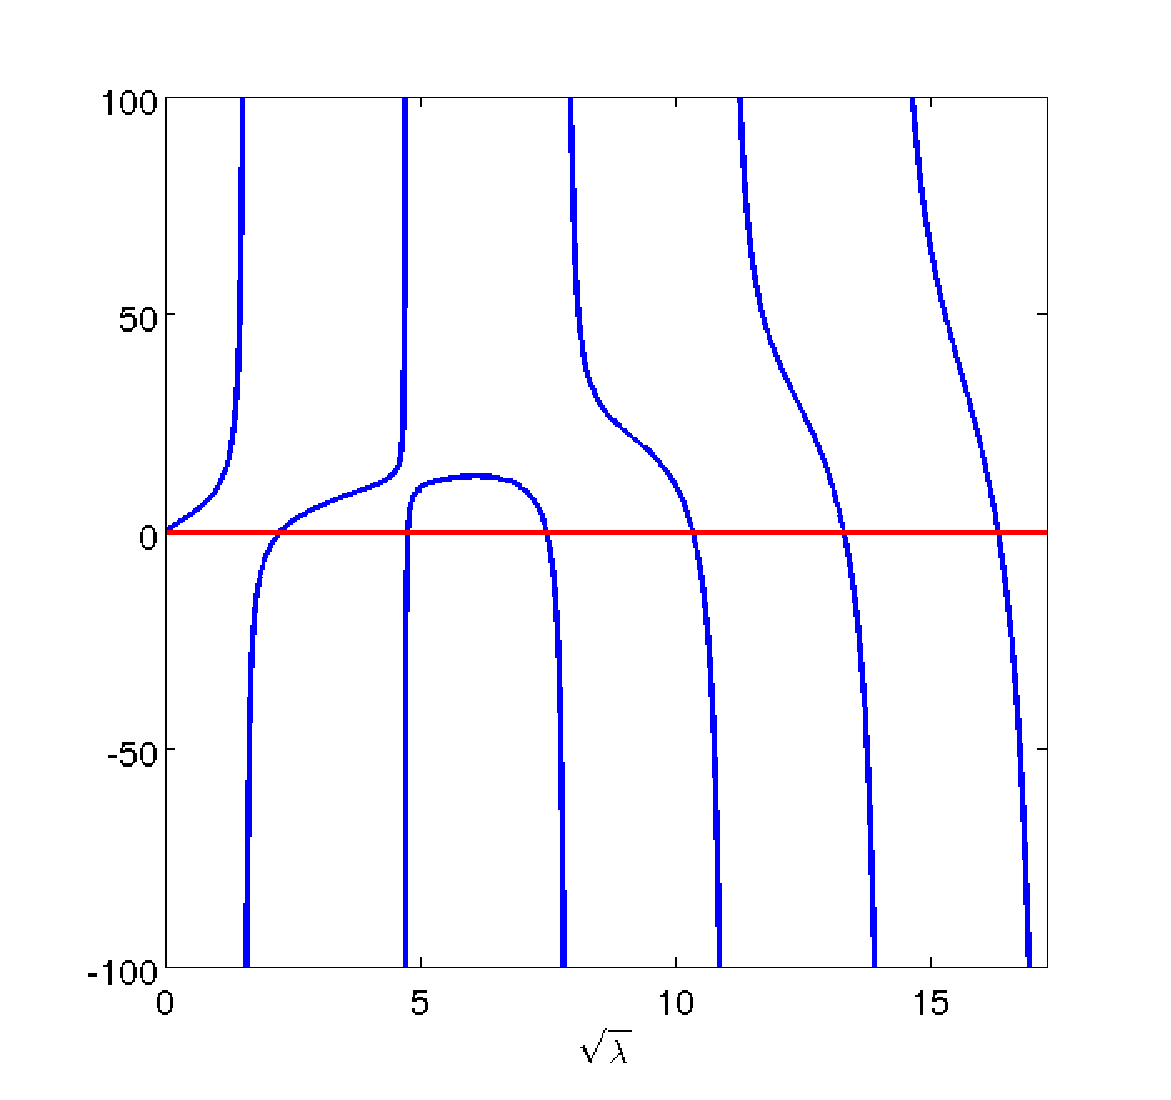
\includegraphics[scale=0.3,trim=1cm 1cm 1cm 1cm,clip=true]{Varie/ricercazeri}
 \end{figure}
\begin{center}Ricerca degli zeri con condizioni di Robin\end{center}
\end{column}
 \end{columns}
\end{frame}
\begin{frame}
 \frametitle{Polimorfismo su \texttt{Basis1DAbstract}...}
 \framesubtitle{... e su \texttt{EducatedBasisFunctorAbstract}}
 \begin{columns}
  \begin{column}{0.5\textwidth}
 \begin{figure}
  \centering
  {\linkimage{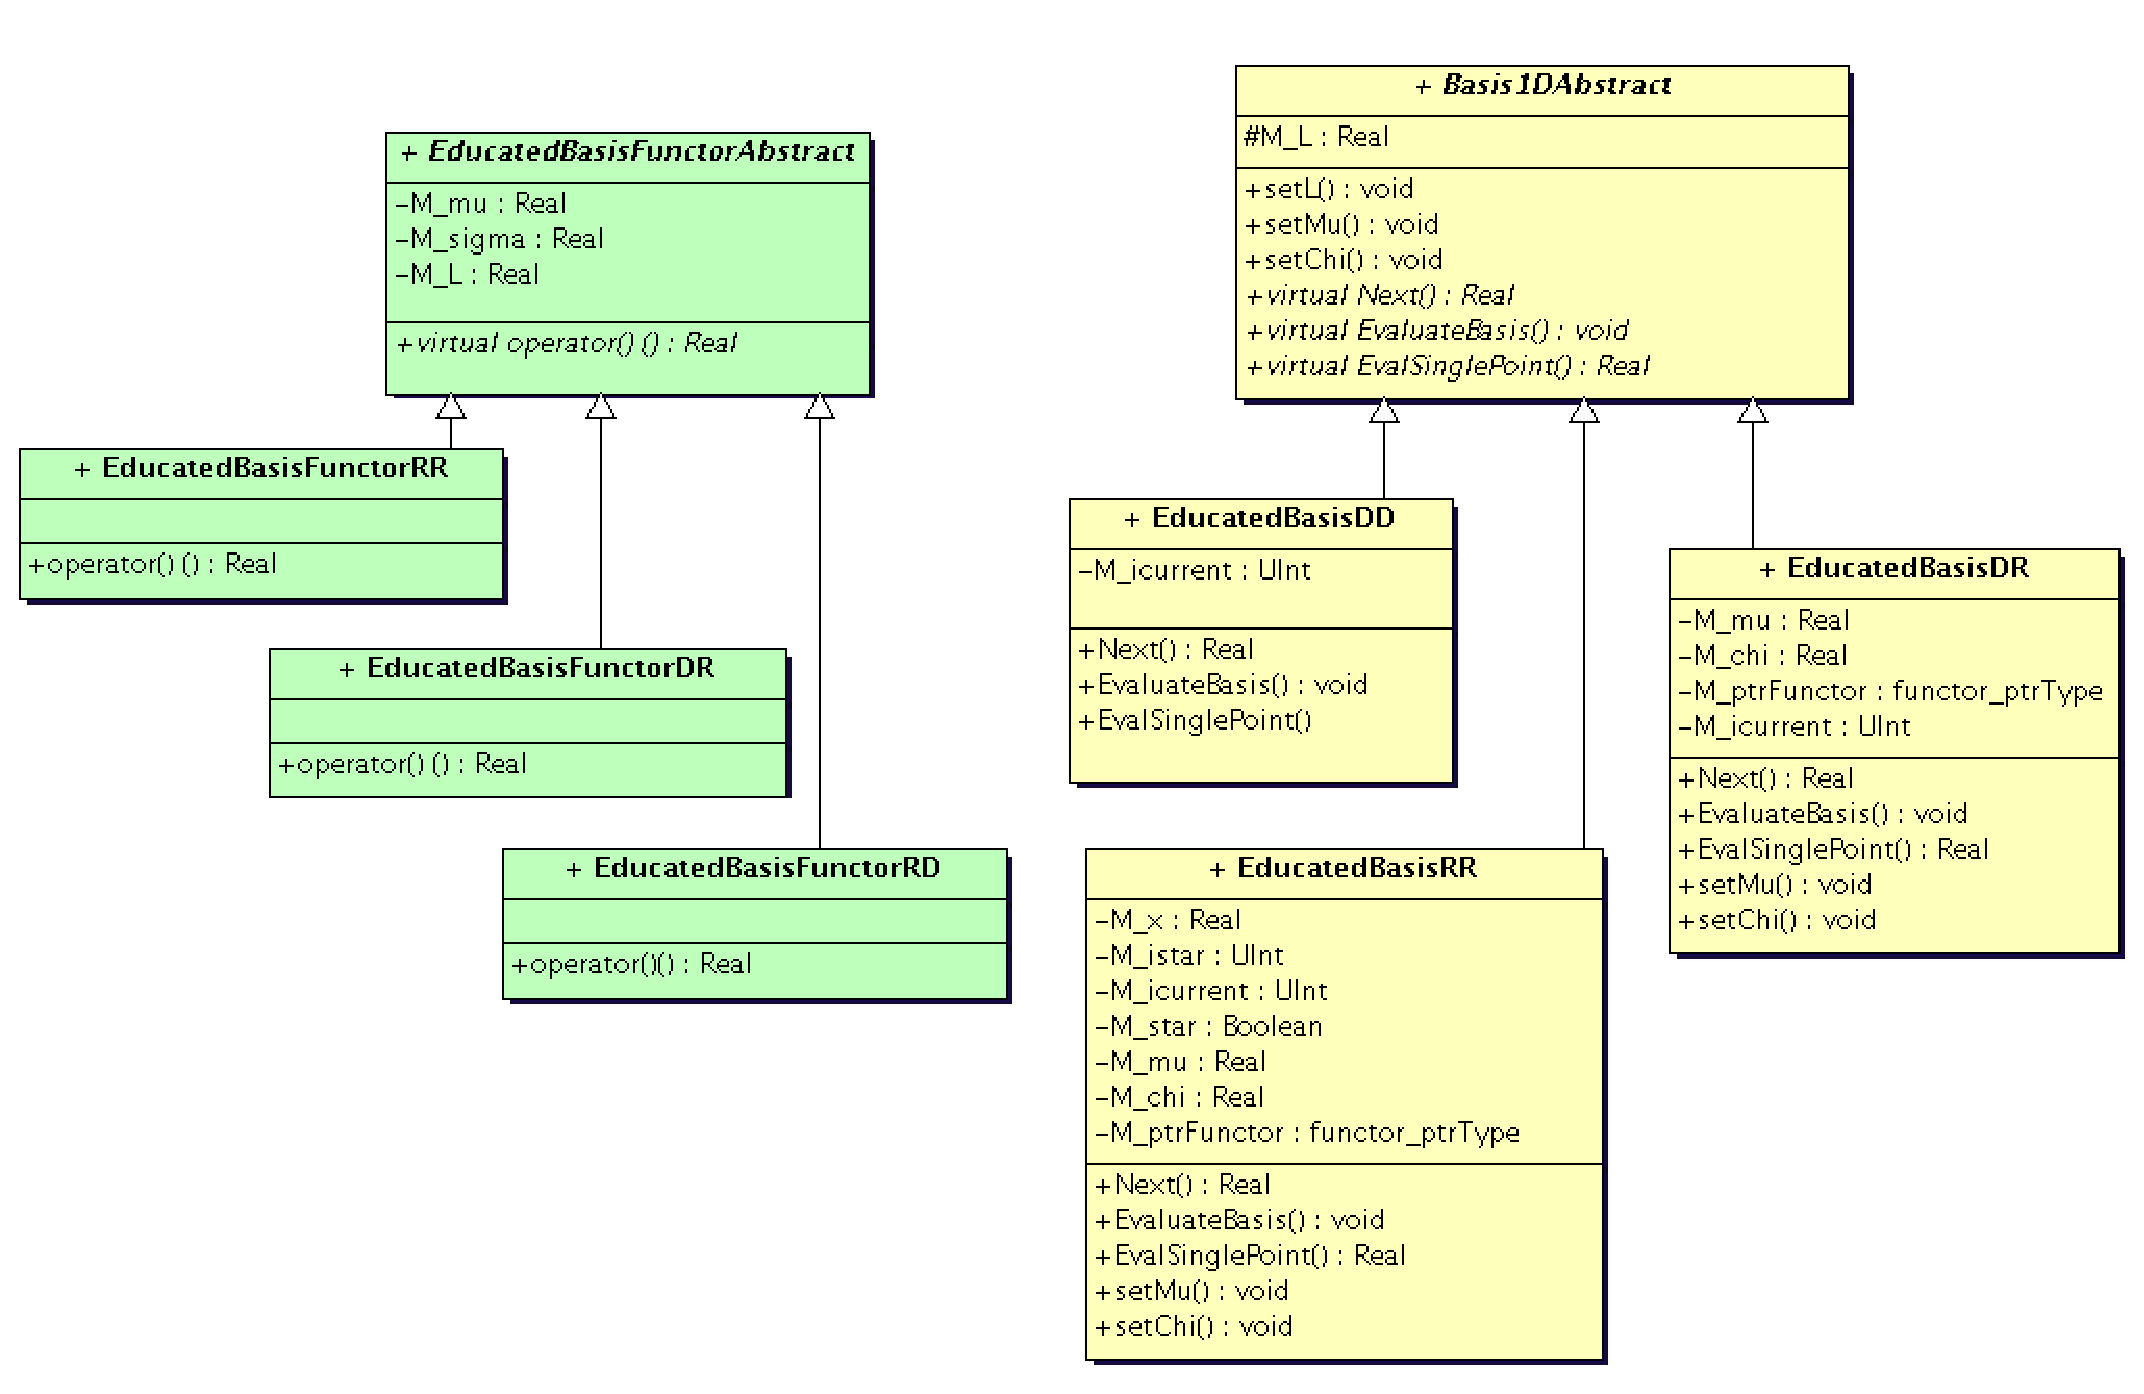
\includegraphics[scale=0.2]{UML/Basis1DAbstract}}{UML/Basis1DAbstract}}
 \end{figure}
  \end{column}
  \begin{column}{0.5\textwidth}
   Per gestire le diverse classi figlie di \texttt{Basis1DAbstract} abbiamo utilizzato una \textbf{factory}.
  \end{column}
 \end{columns}
\end{frame}

\subsection{ModalSpace}

\begin{frame}
\tableofcontents[currentsection]
\end{frame}

\begin{frame}
 \frametitle{\texttt{ModalSpace}}
 \framesubtitle{Una classe che gestisce la costruzione dell'intera base modale}
 \begin{itemize}
  \item Gestisce le formule di quadratura sulla slice
  \item Istanzia i corretti generatori di base\\
  $\rightarrow$ \texttt{AddSliceBC(...)}
  \item Calcola gli autovalori del problema 2D\\
  $\rightarrow$ \texttt{EigensProvider(...)}
  \item Valuta le funzioni di base e le loro derivate nei nodi di quadratura\\
  $\rightarrow$ \texttt{EvaluateBasis(...)}
  \item Calcola i coefficient $r^{st}_{k,j}$\\
  $\rightarrow$ \texttt{Compute\_*(...)}
 \end{itemize}
\end{frame}
\begin{frame}[fragile]
\frametitle{\texttt{AddSliceBC(...)}}
\framesubtitle{due metodi uno per ogni direzione}
\begin{lstlisting}[style = general]
void ModalSpace::
AddSliceBCY (const string& left, const string& right, const Real& mu, const Real& chi)
{
	// Creation of the correct basis generator
	M_genbasisY = Basis1DFactory::istance().createObject(left+right);
	// Setting of the parameters
	M_genbasisY->setL(M_Ly);
	M_genbasisY->setMu(mu);
	M_genbasisY->setChi(chi);
	return;
}
\end{lstlisting}
\end{frame}

\begin{frame}
\frametitle{EigensProvider()}
\framesubtitle{Ordinare correttamente gli autovalori non \`e facile}
\begin{tikzpicture}
[scale=1.5]
\footnotesize
\tikzstyle{eig}=[rectangle, draw, fill=blue!20];
\tikzstyle{temp}=[rectangle,draw,fill=yellow!20];
\tikzstyle{rip}=[rectangle,draw,fill=red!70];
\def\yo{4.8}
\def\dy{-1}
\def\c{1.5}
\def\spazio{2}
\useasboundingbox (-4,0) rectangle (4,5);
\node<1->[eig] (v1) at (0,\yo)  {$(1,0.44)\psp{\spazio}\mathbf{1.44}$};
\node<2-4>[temp] (v2) at (-\c,\yo+\dy)  {$(4,0.44)\psp{\spazio}\mathbf{4.44}$};
\node<2-2>[temp] (v3) at (+\c,\yo+\dy)   {$(1,1.77)\psp{\spazio}\mathbf{2.77}$};
\draw<2->[->] (v1) -- (v2);
\draw<2->[->] (v1) -- (v3);
\node<3->[eig] (v3) at (+\c,\yo+\dy)   {$(1,1.77)\psp{\spazio}\mathbf{2.77}$};
\node<4->[temp] (v4) at (\c - \c/2,\yo+2*\dy) {$(4,1.77)\psp{\spazio}\mathbf{5.77}$};
\node<4-8>[temp] (v5) at (\c + \c/2,\yo+2*\dy) {$(1,4)\psp{\spazio}\mathbf{5}$};
\draw<4->[->] (v3) -- (v4);
\draw<4-8>[->] (v3) -- (v5);
\node<5->[eig] (v2) at (-\c,\yo+\dy) {$(4,0.44)\psp{\spazio}\mathbf{4.44}$};
\node<6->[temp] (v6) at (-\c-\c/2,\yo+2*\dy) {$(9,0.44)\psp{\spazio}\mathbf{9.44}$};
\node<6-6>[temp] (v7) at (-\c+\c/2,\yo+2*\dy) {$(4,1.77)\psp{\spazio}\mathbf{5.77}$};
\draw<6->[->] (v2) -- (v6);
\draw<6->[->] (v2) -- (v7);
\node<7->[rip] (v7) at (-\c+\c/2,\yo+2*\dy) {$(4,1.77)\psp{\spazio}\mathbf{5.77}$};
\node<8->[eig] (v5) at (\c + \c/2,\yo+2*\dy) {$(1,4)\psp{\spazio}\mathbf{5}$};

\def\s{-0.5}
\def\sp{0.3}
\node<1->[eig] (legeig) at (-4+\sp,\s+\yo+2.3*\dy) {$\psp{5}$};
\node<1->[right,text width=11.5cm] (texteig) at (-3.5,\s+\yo+2.3*\dy) {Nodi gi\`a salvati in \texttt{M\_eigenvalues}, 
\`e un \texttt{vector} il cui indice, k \`e gi\`a associato all k-esima \textbf{frequenza}.};
\node<2->[temp] (legtmp) at (-4+\sp,\s+\yo+3.2*\dy) {$\psp{5}$};
\node<2->[right,text width=11.5cm] (texteig) at (-3.5,\s+\yo+3.2*\dy) {Nodi temporaneamente salvati in un \texttt{set}.\\ Esso, grazie ad un'%
opportuna \textbf{relazione d'ordine}, \`e in grado di evitare i doppioni, senza rimuovere gli autovalori doppi e mantenendo 
sempre in prima posizione l'autovalore pi\`u piccolo pronto per l'estrazione.};
\node<7->[rip] (legrip) at (-4+\sp,\s+\yo+4.1*\dy) {$\psp{5}$};
\node<7->[right,text width=11.5cm] (texteig) at (-3.5,\s+\yo+4.1*\dy) {Nodi doppi \textbf{esclusi} dal \texttt{set} perch\'e gi\`a presenti nell'albero.};
\end{tikzpicture}
\end{frame}

\begin{frame}[fragile]
\frametitle{\texttt{EvaluateBasis(...)}}
\framesubtitle{Valutare le funzioni di base sui nodi di quadratura}
\begin{lstlisting}[style=general]
void ModalSpace::
EvaluateBasis()
{
    // Compute all the eigens from the 1D problems
    EigensProvider();
    
    // Fill the matrices with the evaluation of 
    // the monodimensional basis and its derivatives
    M_genbasisY->EvaluateBasis (M_phiy, M_dphiy, 
                                M_eigenvaluesY, M_quadruleY);
    M_genbasisZ->EvaluateBasis (M_phiz, M_dphiz, 
                                M_eigenvaluesZ, M_quadruleZ);
}
\end{lstlisting}
\end{frame}
\begin{frame}[fragile]
 \frametitle{\texttt{Compute\_*(..)}}
 \framesubtitle{Sfruttando la separazione di variabili}
 \begin{lstlisting}[style=general]
Real ModalSpace::
Compute_PhiPhi (const UInt& j, const UInt& k) const
{   //... 
    //... (Date le frequenze estrae i sottoindici p e q)
    for (UInt n = 0; n < M_quadruleY->nbQuadPt(); ++n)
    coeff_y += M_phiy [p_j][n] * normy *
                   M_phiy [p_k][n] * normy *
                   M_Ly * M_quadruleY->weight (n);
    for (UInt n = 0; n < M_quadruleZ->nbQuadPt(); ++n)
    coeff_z += M_phiz[q_j][n] * normz *
                   M_phiz[q_k][n] * normz *
                   M_Lz * M_quadruleZ->weight (n);
    return coeff_y * coeff_z;
}
\end{lstlisting}

{\footnotesize\textbf{\red{WIP}}: Abbiamo aggiunto dei metodi per considerare 
\textbf{coefficienti non costanti} che si occupano di calcolare i coefficienti $r^{st}_{j,k}$ \textbf{senza separare le variabili}.

Sono ancora da testare e da ottimizzare.}
\end{frame}

\subsection{HiModAssembler}

\begin{frame}
\tableofcontents[currentsection]
\end{frame}

\begin{frame}
 \frametitle{HiModAssembler}
 \framesubtitle{La classe che combina gli elementi finiti e la base modale}
 \begin{itemize}
  \item \textbf{Membri principali}
  \begin{itemize}
   \item \texttt{M\_modalbasis}
   \item \texttt{M\_etfespace}
  \end{itemize}

  \item Metodi per l'\textbf{assemblaggio}
  \begin{itemize}
   \item \texttt{AddADRProblem(...)}
   \item \texttt{interpolate(...)}
   \item \texttt{Addrhs(...)}
   \item \texttt{AddDirichletBC\_In(...)}
  \end{itemize}

  \item Metodi per l'\textbf{analisi}
  \begin{itemize}
   \item \texttt{evaluateBase3DGrid(...)} \textcolor{green!50!black}{$//$HiMod vector}
   \item \texttt{evaluateBase3DGrid(...)} \textcolor{green!50!black}{$//$Function type}
   \item \texttt{normL2(...)}
  \end{itemize}

  \item Metodi per l'\textbf{export}
  \begin{itemize}
   \item \texttt{ExportStructuredVTK(...)}
   \item \texttt{ExportFunctionVTK(...)}
  \end{itemize}

 \end{itemize}

\end{frame}
\begin{frame}[fragile]
 \frametitle{\texttt{AddADRProblem(...)}}
 \framesubtitle{Utilizzo del pacchetto ETA per assemblare i problemi 1D}
 \begin{lstlisting}[style=general]
for j {
for k {
VectorSmall<5> Coeff;
Coeff[0] = M_modalbasis->Compute_PhiPhi (j, k);
//...
{ using namespace ExpressionAssembly;
  //...
  integrate(
      elements(M_etfespace->mesh()),
      M_fespace->qr(),
      M_etfespace,
      M_etfespace,
      mu*Coeff[0]*dot(grad(phi_i),grad(phi_j))
      //...
      )
  >>(systemMatrix->block(k,j));
}
//...
return;
\end{lstlisting}
\end{frame}
\chapter{Risultati}
In questa sezione mostreremo alcuni dei risultati che abbiamo ottenuto, per visualizzarli abbiamo utilizzato
il software ParaView.
All'interno del file \texttt{himod/util/CaseTest.hpp} sono salvati diversi casi test
con soluzione esatta e uno senza (la forzante \`e stata ottenuta usando il symbolic toolbox di Matlab).
Nel caso si fosse interessati ad aggiungere altri casi test \`e possibile aggiungerli modificando i
file \texttt{CaseTest.hpp} e \texttt{CaseTest.cpp}. Una volta creato il caso test 
occorre aggiungerlo allo switch che si trova nella classe \classe{GeneralTest} nella
cartella \texttt{util}. \classe{GeneralTest} \`e una classe che abbiamo sviluppato per poter
lanciare diversi test senza dover modificare il sorgente, ma semplicimente settando 
parametri  e caso test dal datafile di \texttt{GetPot}\footnote{Se si vuole provare a lanciare qualche test si veda il tutorial
\texttt{4\_generaltest}, se invece si vuole vedere come si dovrebbe assemblare un test da zero si veda il tutorial \texttt{1\_ADR} }.
Cominciamo mostrando il caso test senza soluzione esatta, che per\`o \`e pi\`u interessante dal punto di vista qualitativo.
\begin{equation}
 \label{eq:camini}
 \left\{
\begin{aligned}
 &-\Delta u + \vect{\beta}\cdot\nabla u + \sigma u = f &\quad \text{ in }\Omega=(0,2)\times(0,1)\times(0,1)\\
 &u=0 &\quad \text{ su } \Gamma_{in} \cup \Gamma_{lat}\\
 &\nabla u\cdot \vect{n} = 0 &\quad \text{ su } \Gamma_{out},
\end{aligned}
\right.
\end{equation}
dove $\vect{\beta}=(5,1,0)$, $\sigma=0.3$ e $f$ \`e riportata in figura \ref{fig:fcamini}.
In figura \ref{fig:confrontocamini} abbiamo sulla sinistra la soluzione ottenuta con 
gli elementi finiti (sempre con LifeV), utilizzando una griglia strutturata con \# elementi in direzione $x$
e \# in direzione $y$ e $z$, sulla destra invece c'\`e la soluzione ottenuta con HiMod, \# elementi in direzioni $x$
e 50 modi. Osserviamo che 50 modi, in un problema come questo dove la geometria e le condizioni al bordo sono le stesse in direzione
$x$ e $y$, significa circa 7 modi in direzione $y$ e altrettanti in direzione $z$.
Vediamo come, dal punto di vista qualitativo, il fenomeno venga colto bene anche dalla riduzione gerarchica di modello.
Nella figura \ref{fig:camini2d+} vediamo diverse sezioni trasversali del dominio e possiamo apprezzare, sempre dal punto di vista qualitativo,
la convergenza. Vediamo che gi\`a con 9 modi la soluzione \`e ragionevole anche se non \`e in grado di cogliere 
bene tutte le caratteristiche della soluzione, con 16 modi ci sono evidenti miglioramenti e con 25 siamo gi\`a a convergenza dal punto di 
vista qualitativo, non abbiamo quindi riportato risultati con pi\`u di 25 modi.
Infine, in figura \ref{fig:camini2D}, riportiamo un'altra visualizzazione di una sezione orizzontale con $y=0.5$.
Anche qui possiamo apprezzare la convergenza.
Nei successivi esperimenti abbiamo testato diverse combinazioni di dati al bordo e abbiamo cercato di verificare la convergenza del 
metodo. 
\subsection*{Convergenza}
Dal punto di vista teorico la teoria della convergenza per le basi istruite \`e ancora in fase di sviluppo.

Nel caso 2D si ha una convergenza di ordine due in $L^2(\Omega)$ rispetto al numero di modi.
In particolare nel caso Dirichlet in 2D usando i P1 in direzione $x$ si ha per $u\in H^2(\Omega)$
\begin{equation}
 \label{eq:stimainl2}
 ||u-u_{m,h}||_{L^2(\Omega)}\leq C ( h^2+m^{-2}) ||u||_{H^2},
\end{equation}
per maggiori dettagli su questo caso si possono trovare in \cite{zilio:himod} teoremi 3.15 e 3.16.

In 3D tenendo conto che $m\sim m_y\cdot m_x$ e con altre considerazioni basate sulle propriet\`a del problema agli autovalori
\`e ragionevole aspettarsi un ordine uno in $L^2(\Omega)$ rispetto al numero di modi, ma la dimostrazione 
non \`e stata ancora terminata.

Nella figura \ref{fig:ddddconv} possiamo vedere un caso test con condizioni di Dirichlet sul bordo laterale. Vediamo 
come l'ordine di convergenza sia pari a uno. Vediamo anche che se si usa una griglia elementi finiti troppo 
lasca ad un certo punto l'errore non decresce pi\`u al crescere del numero di modi, perch\`e 
l'errore elementi finiti \`e superiore a quello di modello dovuto all'approssimazione modale.
Vediamo per\`o che riducendo il passo della griglia le curve dell'errore si attestano tutte sulla stessa linea.
Nel caso riportato in figura \ref{fig:drdrconv} abbiamo un caso test con condizioni miste sui lati del quadrato:
il lato in basso e in alto hanno condizioni di Dirichlet, mentre i lati a destra e a sinistra hanno condizioni di Robin.
Anche qui possiamo vedere come il grafico di convergenza confermi i risultati attesi dalla teoria.
Infine abbiamo costruito un caso test con condizioni di Robin su tutti i lati. In figura \ref{fig:rrrr_conv} possiamo 
vedere come l'ordine di convergenza sembra essere superiore alla velocit\`a attesa, questo comportamento in realt\`a 
si verifica anche nei casi test bidimensionali con condizioni al bordo di Robin, dal punto di vista teorico ancora non ci sono 
spiegazioni convincenti, tuttavia questo comportamento si verifica puntualmente.

Abbiamo poi riportato alcuni test per cercare di confrontare gli elementi finiti con HiMod.
In figura \ref{fig:dof} abbiamo riportato il numero di gradi di libert\`a dei due metodi lungo la slice trasversale utilizzati per 
approssimare il caso test con condizioni di Dirichlet che abbiamo utilizzato anche per osservare la convergenza.
Per gli elementi finiti abbiamo utilizzato una griglia strutturata e entrambi i metodi condividono la stessa griglia 
in direzione $x$. Sull'asse delle ordinate abbiamo riportato l'errore in norma $L^2(\Omega)$.
Si vede come a parit\`a di precisione, con himod sia possibile ottenere utilizzare molti meno gradi di libert\`a in direzione trasversale.
Tuttavia questo dipende anche dal caso test, perch\`e l'ordine di convergenza \`e lo stesso, quindi tutto dipende dalla 
costante davanti alla stima dell'errore. \`E chiaro che se la soluzione non presenta dinamiche particolarmente complesse in direzione trasversale,
se la base scelta \`e buona gi\`a con i primi modi si potranno cogliere le caratteristiche principali e dunque la curva HiMod
in figura \ref{fig:dof} si trover\`a al di sotto della curva per gli elementi finiti.

Infine, sempre sul caso test con condizioni di Dirichlet, abbiamo cercato di capire quanto tempo impiega l'assemblaggio della matrice
rispetto all'analogo test assemblato con il pacchetto \texttt{ETA} di \texttt{LifeV}.
I risultati si possono vedere in figura \ref{fig:time} e vediamo come, a parit\`a di precisione, il tempo di assemblaggio 
della matrice sia minore che nel caso elementi finiti, ci\`o \`e dovuto al minor numero di gradi di libert\`a.

% \begin{itemize}
% \item Introduzione teorica
% \item Osservazione sull'influenza dell'errore fem (particolare nel caso RRRR sarebbe da verificare)
% \item Notare la superconvergenza (come da teoria?)
% \end{itemize}
% 
% % \begin{figure}[!htbp]
% %         \centering%
% %         \subfigure[DDDD]%
% %           {\label{fig: convDDDD}\includegraphics[scale=0.25]{Convgopergenze/DDDD_ADR.eps}}\qquad
% %         \subfigure[DRDR]%
% %           {\label{fig:convDRDR}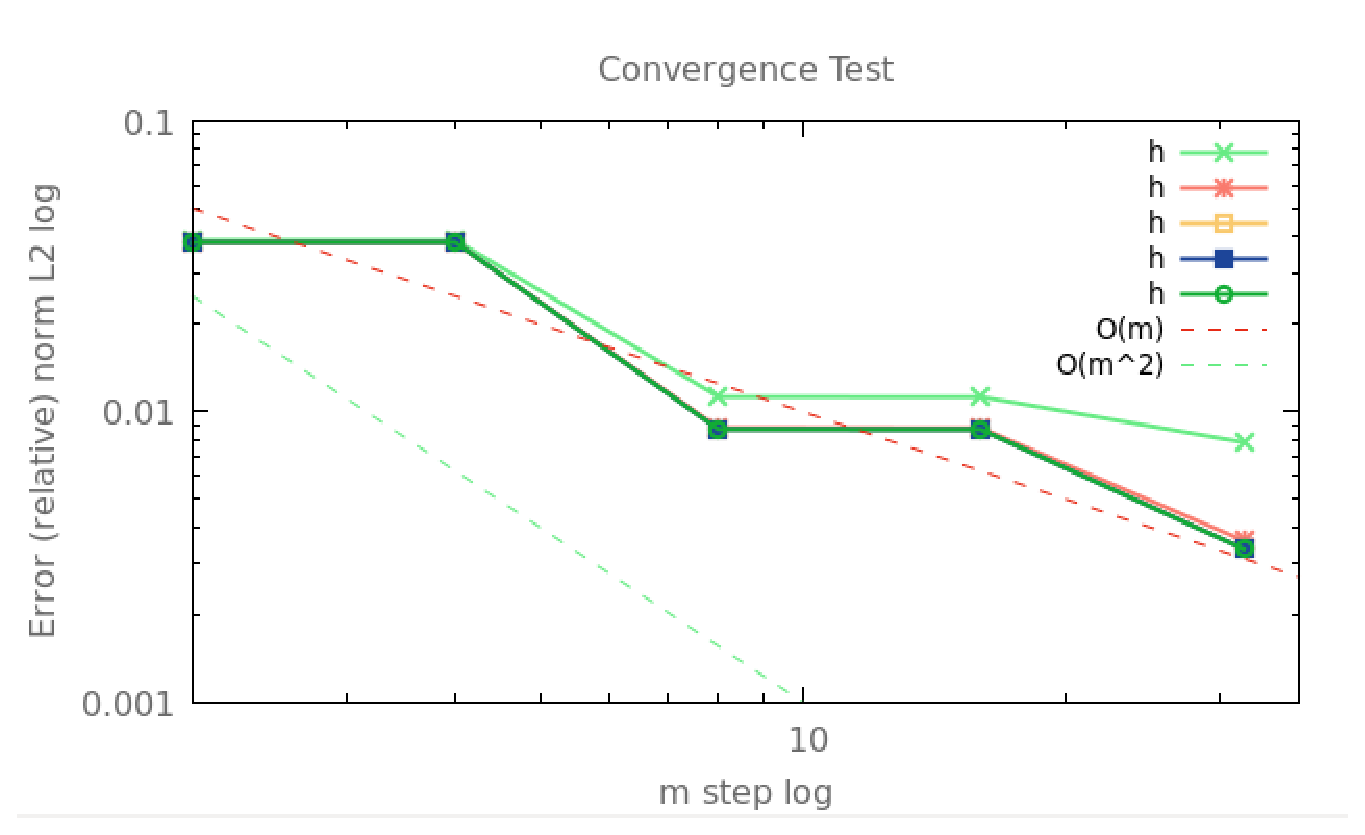
\includegraphics[scale=0.25]{Convergenze/DRDR.eps}}\qquad
% % 		\subfigure[RRRR]%
% %           {\label{fig:convRRRR}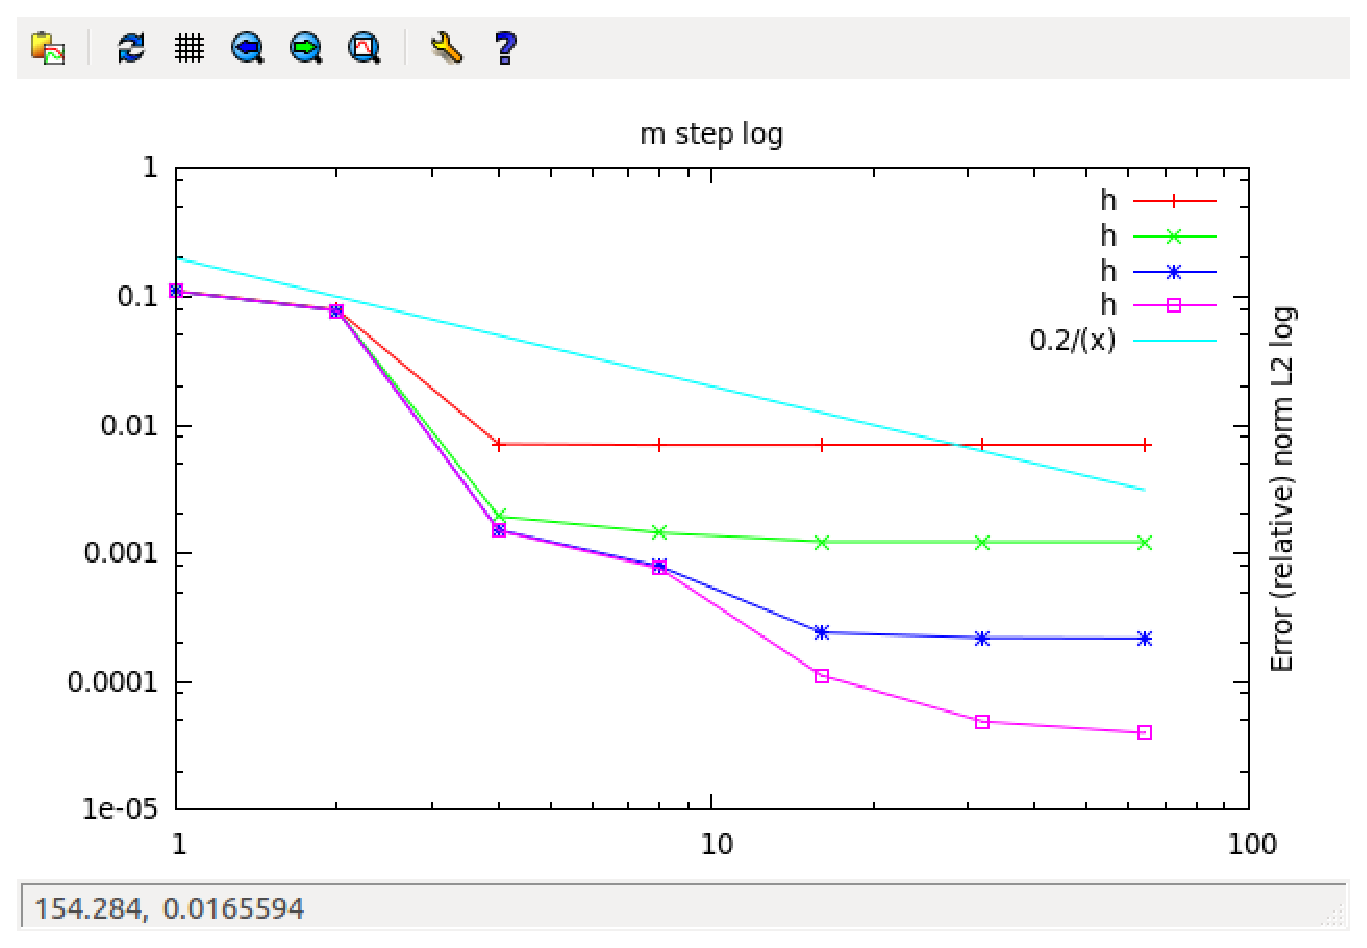
\includegraphics[scale=0.25]{Convergenze/RRRR.eps}}\qquad
% %         \label{fig: convergenze}
% %         \caption{Convergenze casi test}
% % \end{figure}
% 
% \begin{itemize}
% \item Confronto gradi di libert\`a spesi e errore norma L2
% \item Tempo di assemblaggio problema
% \end{itemize}
% \begin{figure}[!h]
% \centering
%           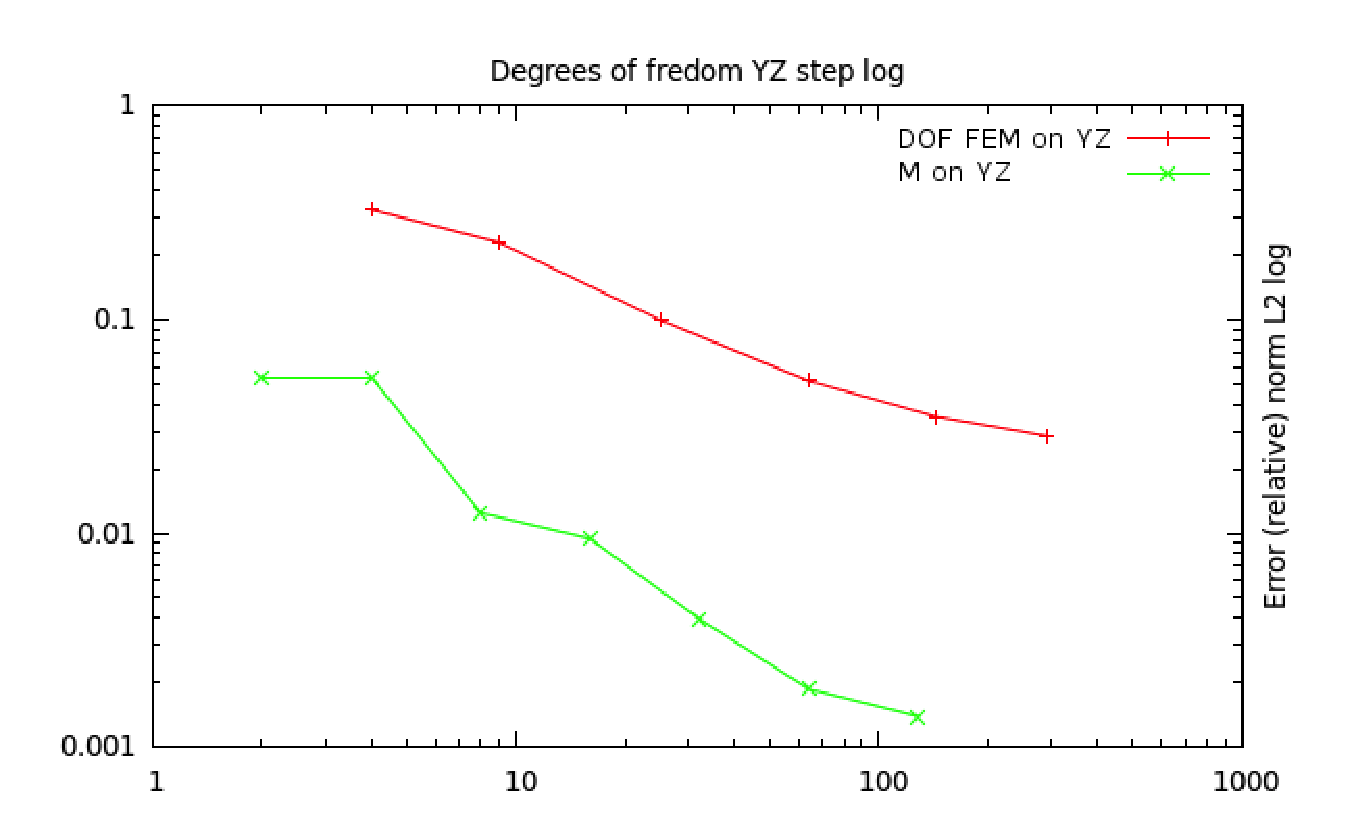
\includegraphics[scale=0.25]{Convergenze/ConfrontoDOF.eps}\qquad
%         \caption{ Confronto DOF}
%         \label{fig: Confronto DOF}
% \end{figure}
% 
% \begin{figure}[!h]
% \centering
%           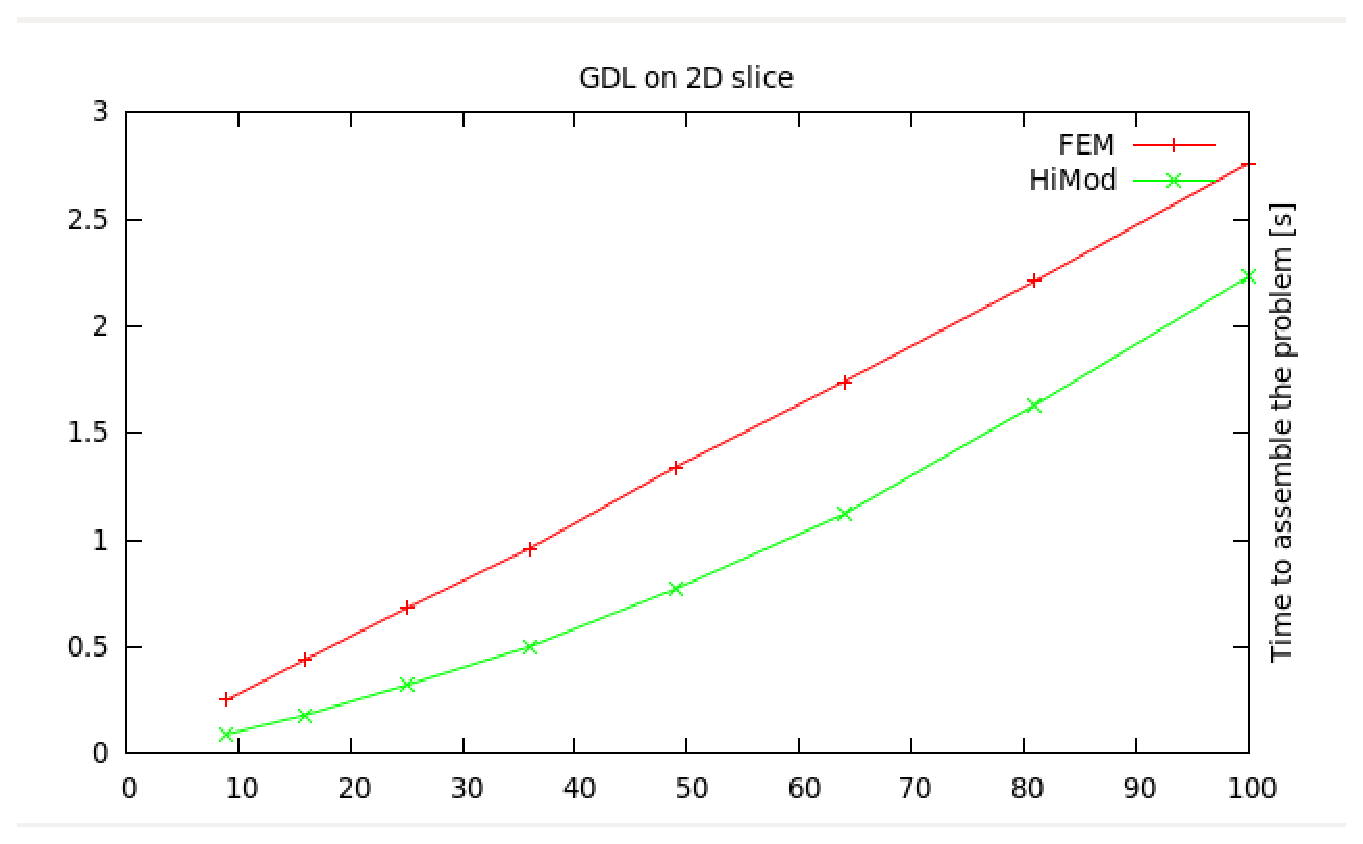
\includegraphics[scale=0.25]{Convergenze/Confronto_tempi.eps}\qquad
%         \caption{ Confronto tempi assemblaggio}
%         \label{fig: Confronto tempi}
% \end{figure}
% 
% \begin{itemize}
% \item Presentazione del caso test
% \item Osservazione sull'aggiunta progressiva di modi (sempre pi\`u frequenze vengono considerate e l'approssimazione cresce)
% \item Commento sui risultati 3D
% \end{itemize}
% 
% \begin{figure}[!htbp]
%         \centering%
%         \subfigure[m=9.]%
%           {\label{fig: slice9}\includegraphics[scale=0.15]{DDDD_ADR/HiMod9slice.eps}}\qquad
%         \subfigure[m=16.]%
%           {\label{fig:slice16}\includegraphics[scale=0.15]{DDDD_ADR/HiMod16slice.eps}}\qquad
% 		\subfigure[m=25.]%
%           {\label{fig:slice25}\includegraphics[scale=0.15]{DDDD_ADR/HiMod25slice.eps}}\qquad
%           \subfigure[FEM.]%
%           {\label{fig:sliceFEM}\includegraphics[scale=0.15]{DDDD_ADR/FEMslice.eps}}\qquad
%         \caption{Caso test DDDD sezione XZ}
%         \label{fig:DDDD_ADR slice}
% \end{figure}
% 
% \begin{figure}[!htbp]
%         \centering%
%                 \subfigure[Forzante e trasporto.]%
%           {\label{fig: force term}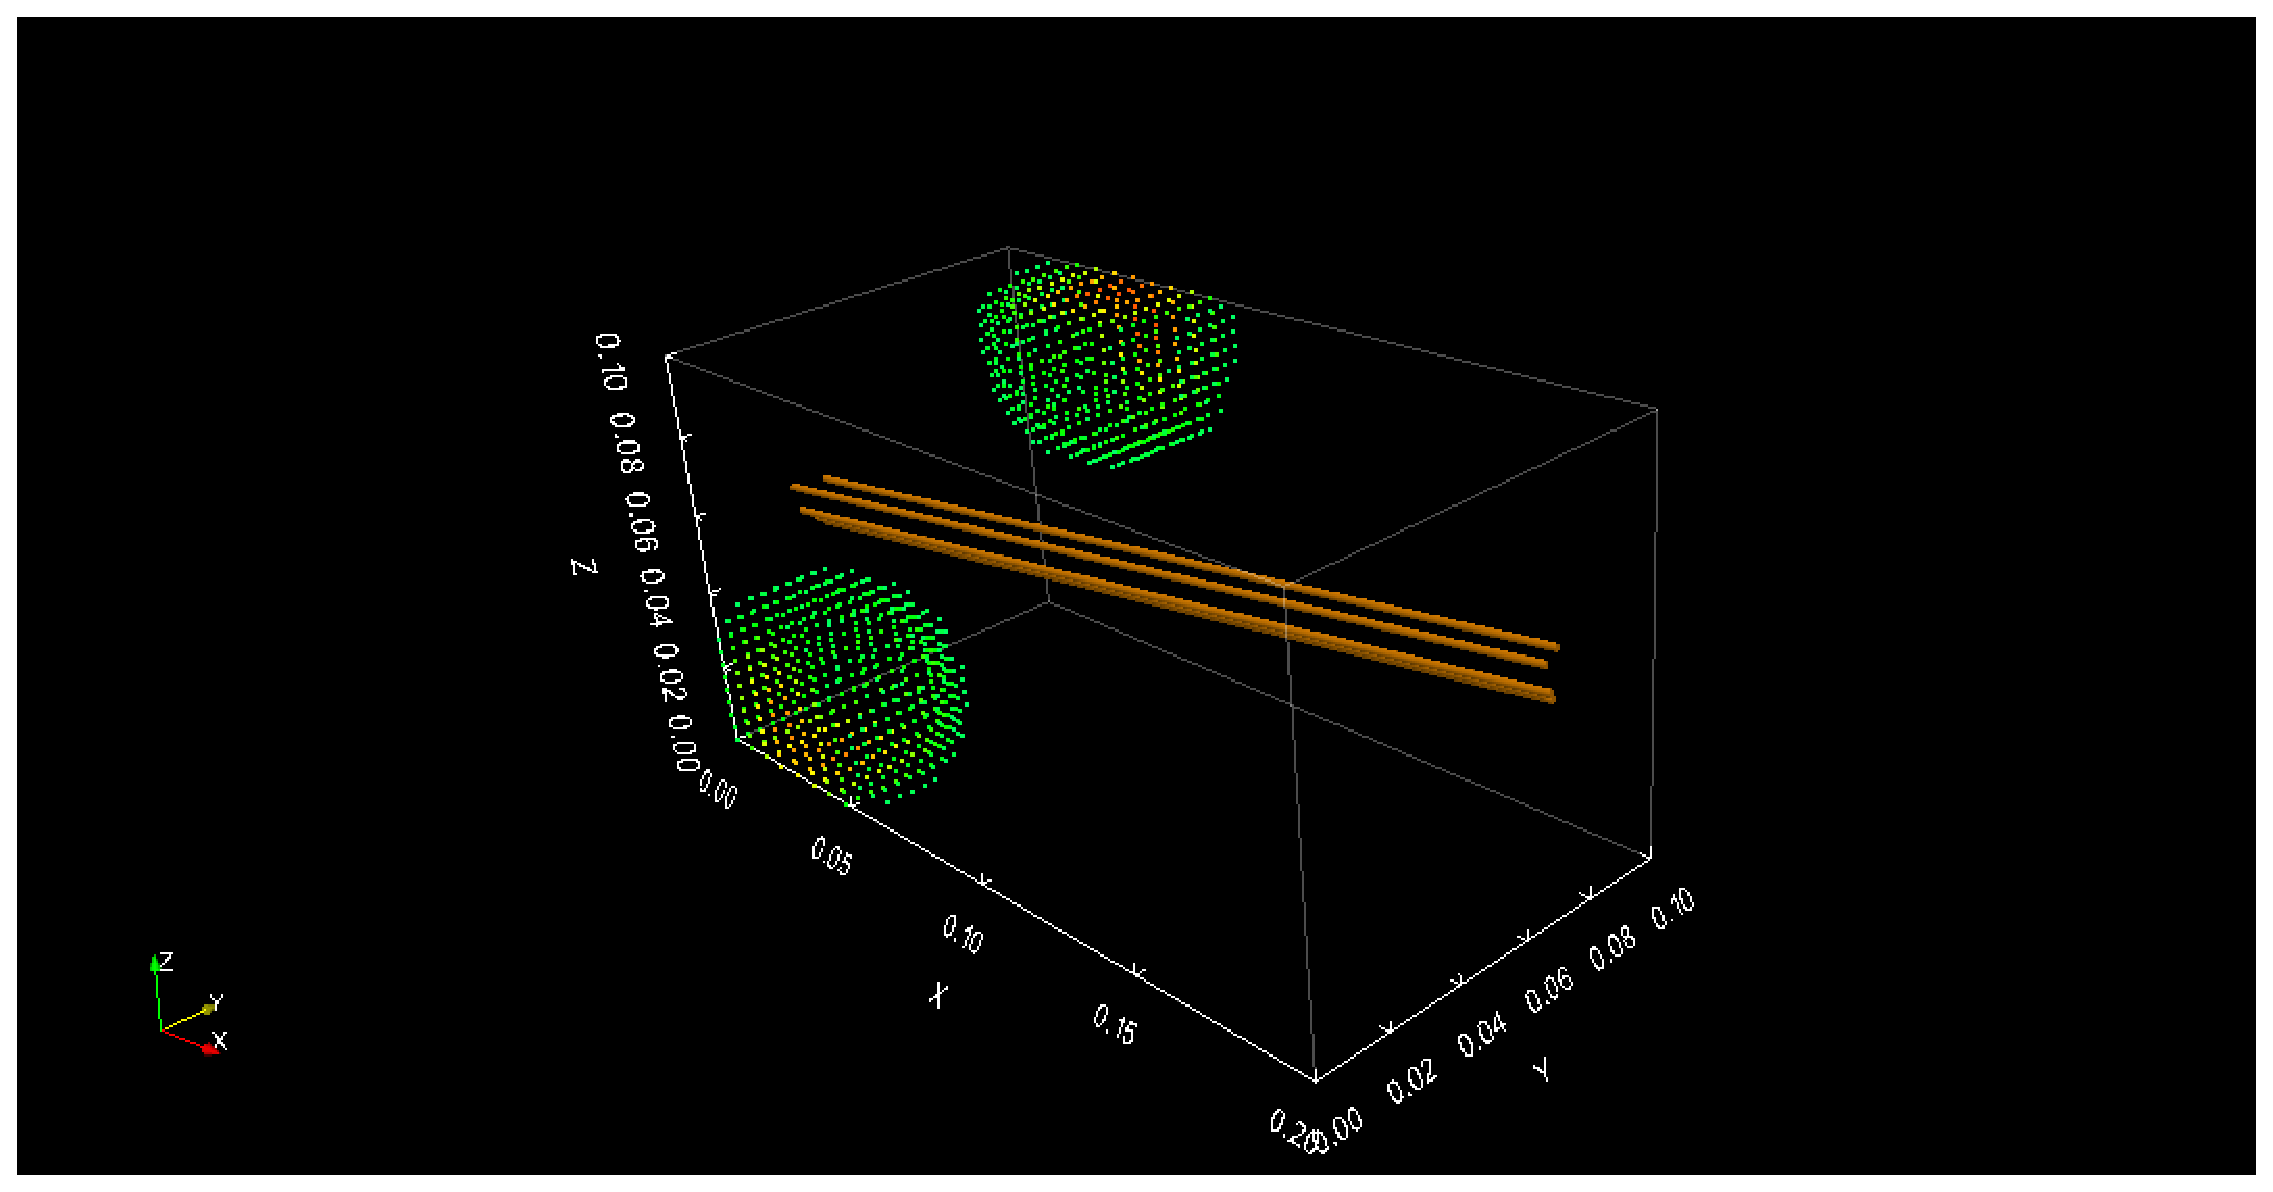
\includegraphics[scale=0.36]{DDDD_ADR/ForcetermTrasport.eps}}\qquad
%         \subfigure[Soluzione FEM.]%
%           {\label{fig: FEMsol}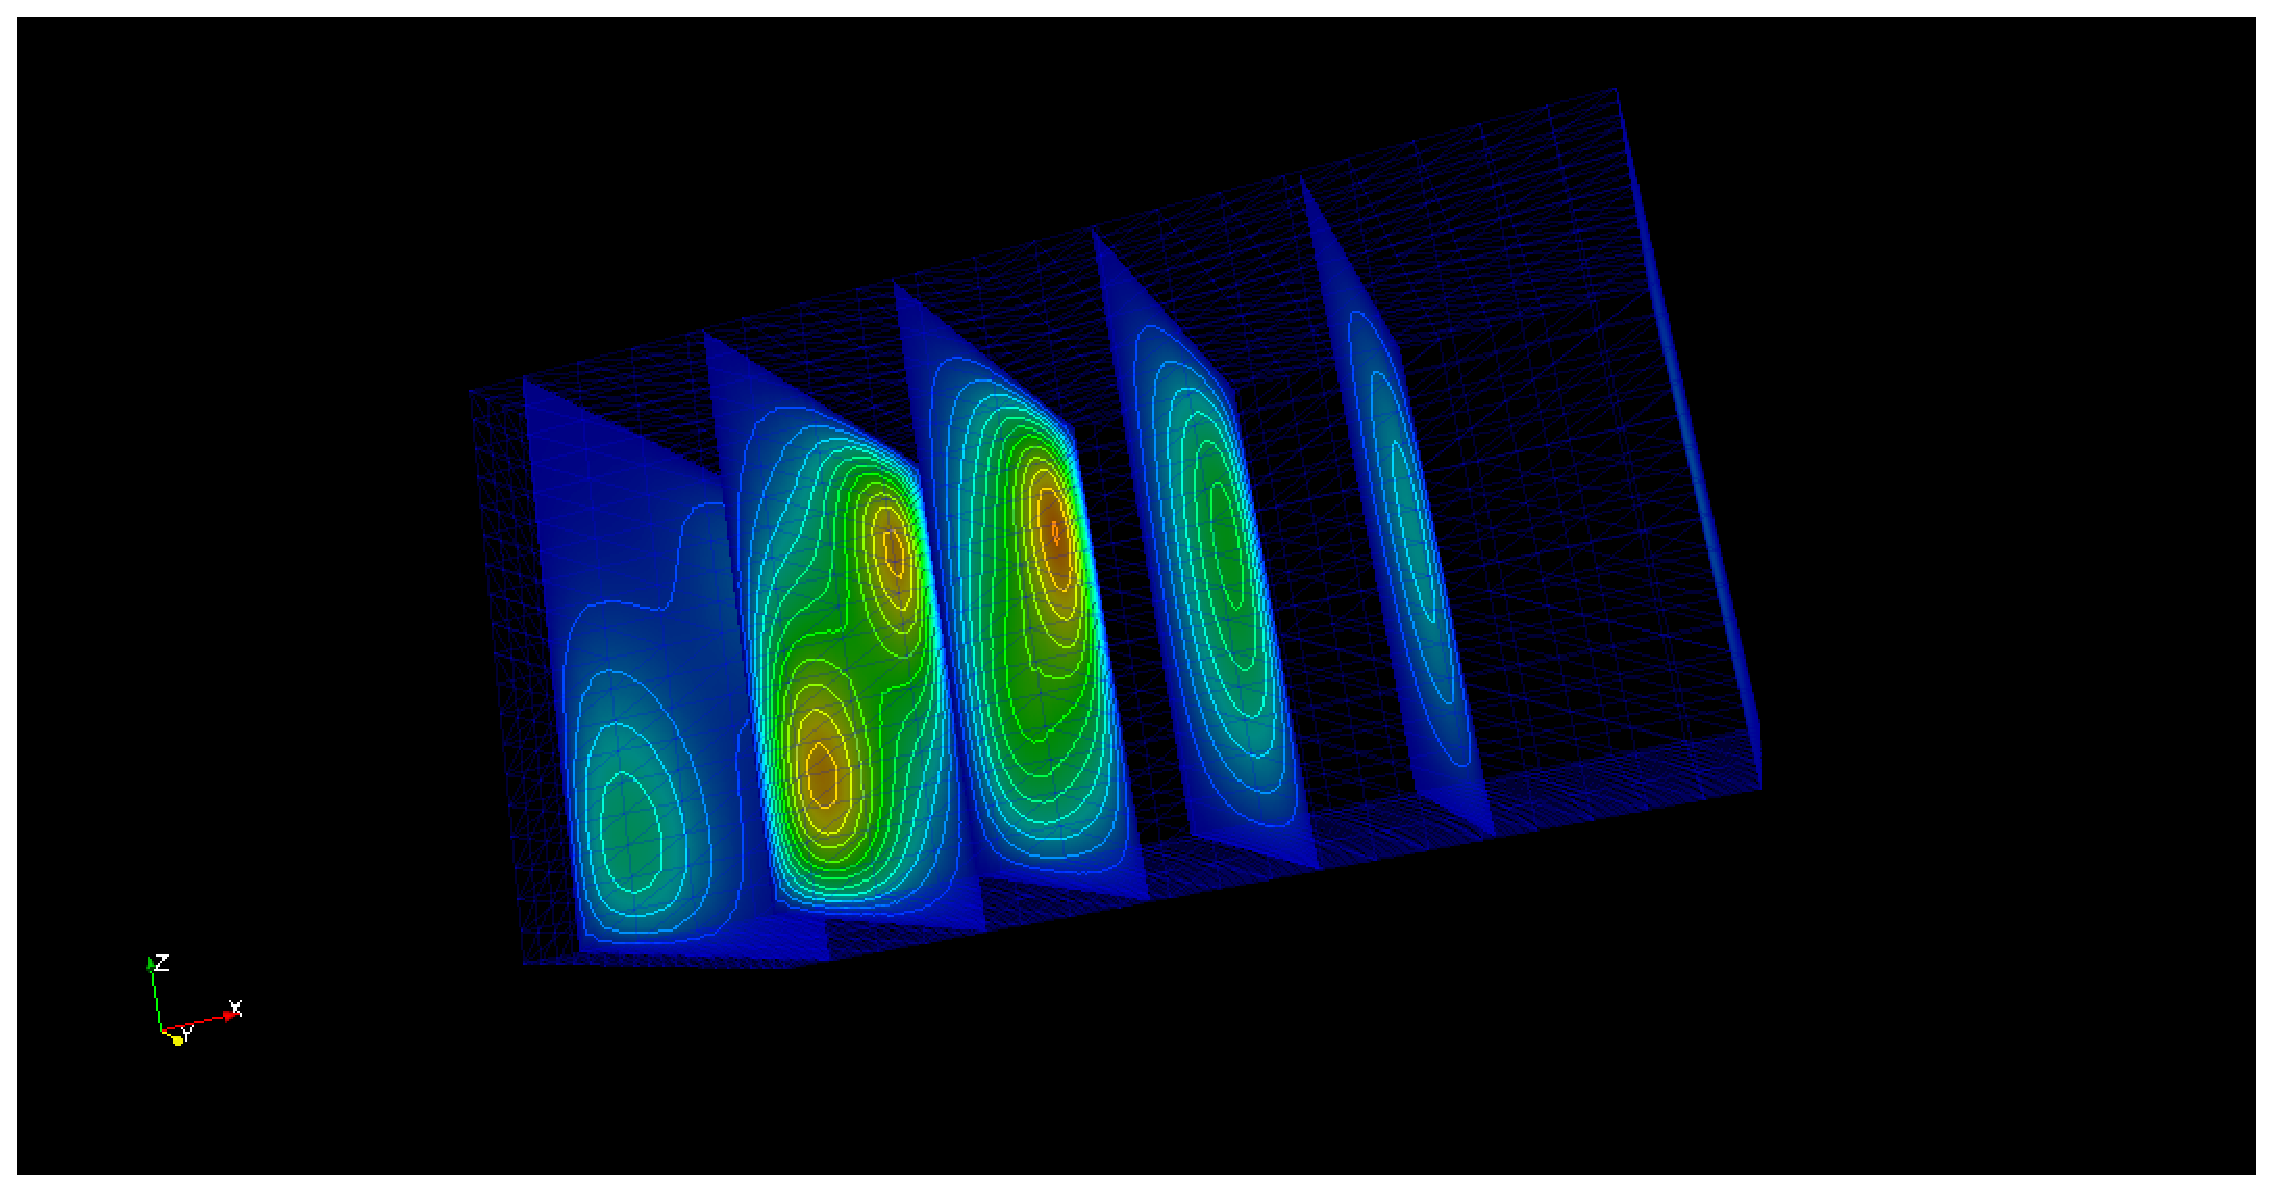
\includegraphics[scale=0.36]{DDDD_ADR/FEM.eps}}\qquad
%         \subfigure[Soluzione HiMod m=50.]%
%           {\label{fig:HiMod50sol}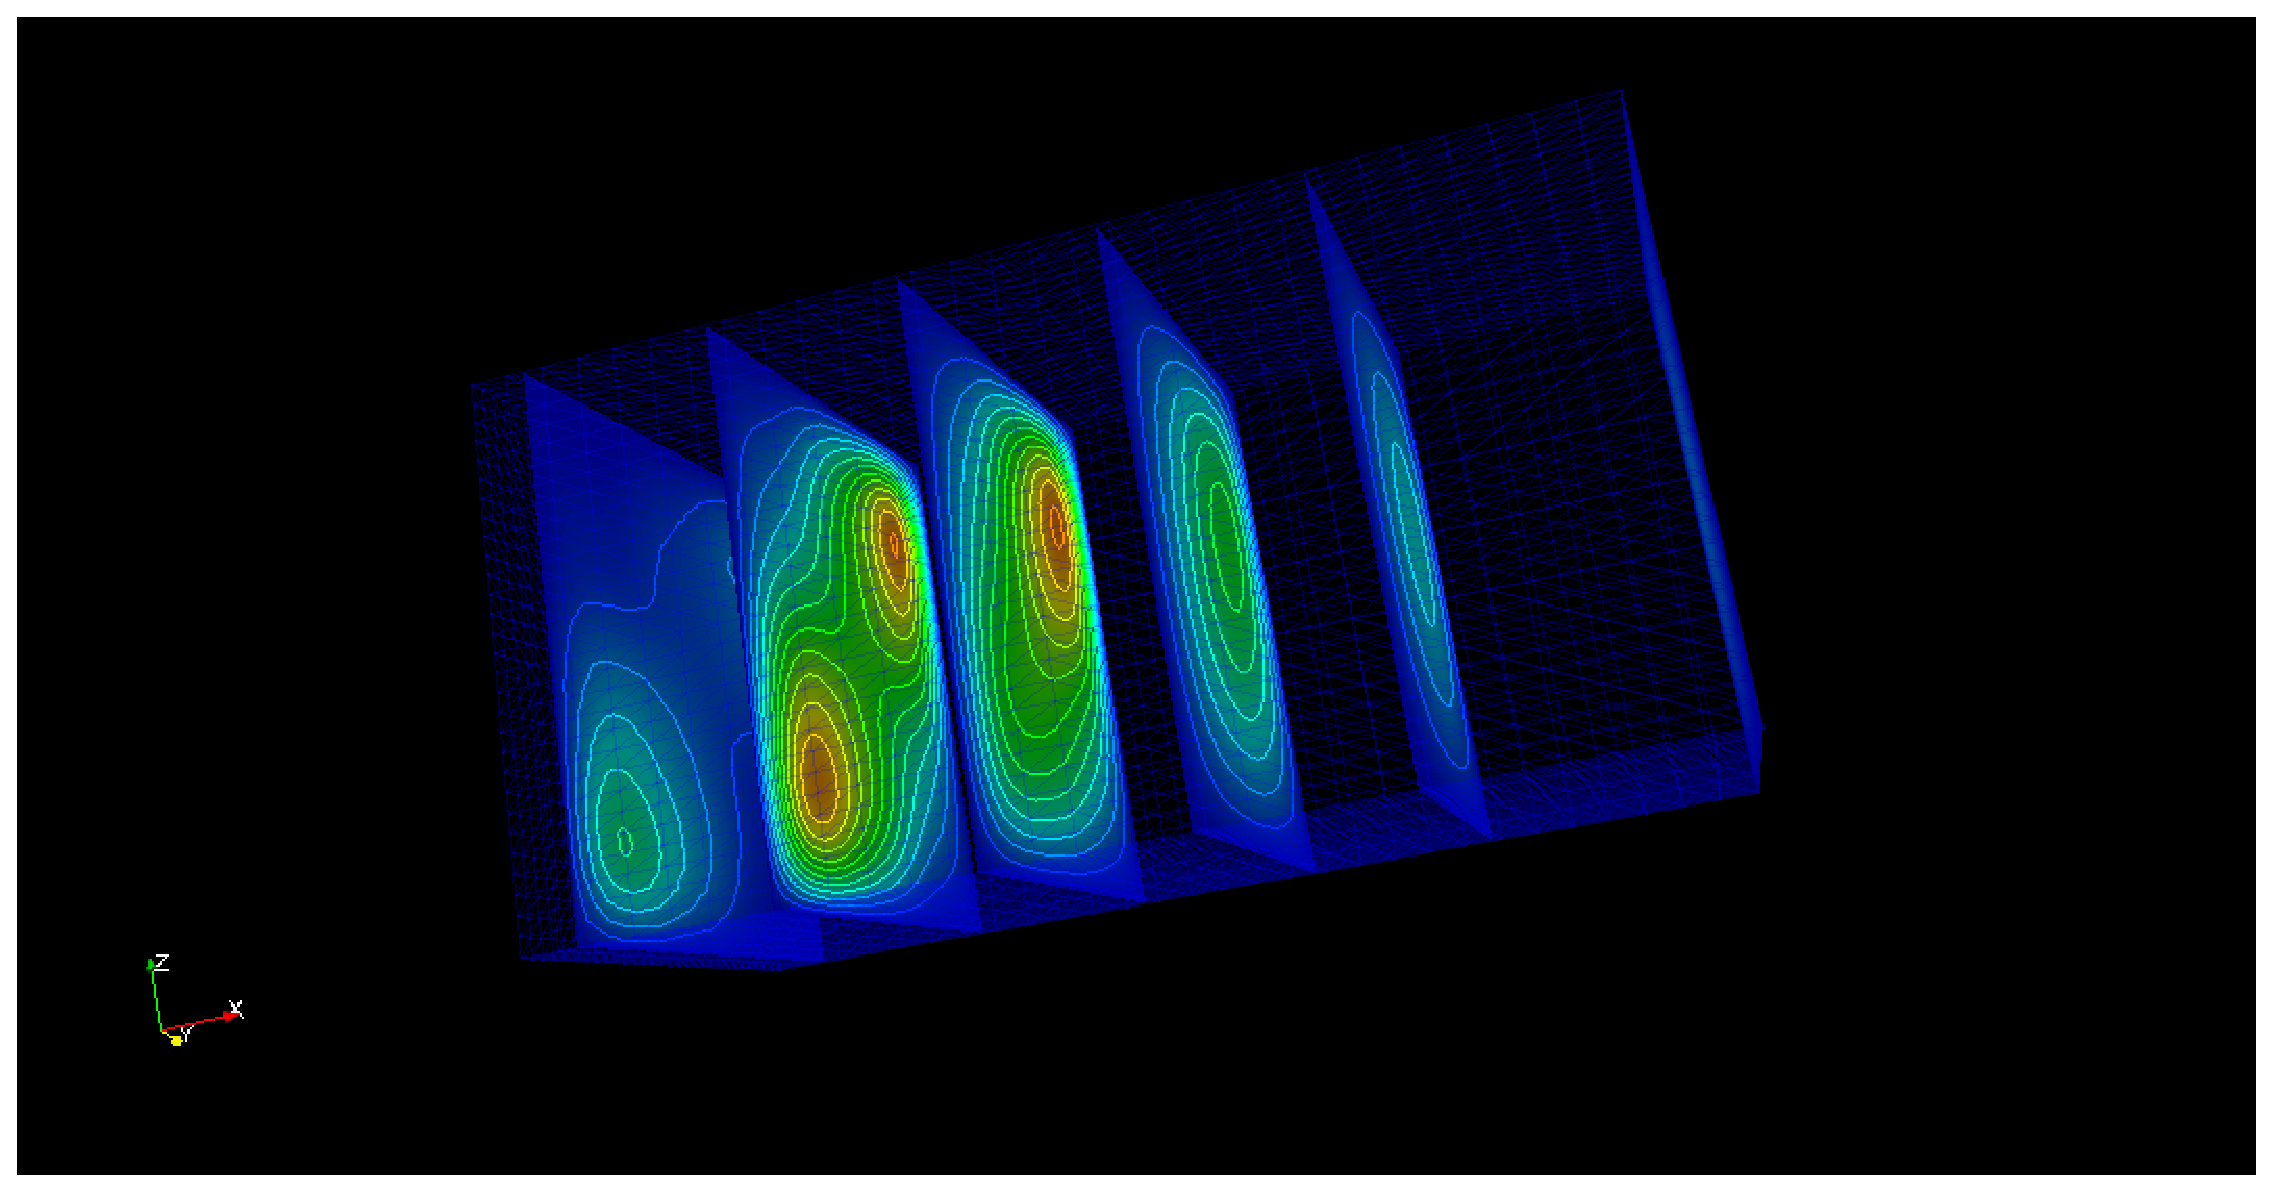
\includegraphics[scale=0.36]{DDDD_ADR/HiMod50.eps}}\qquad
%         \caption{Caso test DDDD\_ADR}
%         \label{fig:DDDD_ADR}
% \end{figure}
\flushlinkimages
\end{document}